%%% Time-stamp: <mainrep.tex 19:57, 17 Jul 2016 by P Sunthar>
%%% $Log:$
% This document describes how to use iitbreport style
%********************************************************************

%\documentclass[11pt,a4paper,openright]{report}
\documentclass[twoside]{iitbreport}

%% Default spacing: 1.5
%% Default font size: 12pt
%% Default font: txfonts (similar to times new roman) 

%% Selectively comment out sections that you want to be left out but
%% maintaining the page numbers and other \ref
\includeonly{%
  pre/preliminaries,
  spw/spw,
  latest/latest,
  dec,ack
}
%%expt/experimental,
%%,pub
%%% Some commonly used packages (make sure your LaTeX installation
%%% contains these packages, if not ask your senior to help installing
%%% the packages)

\usepackage{booktabs}
\usepackage[italicdiff]{physics}
\usepackage{braket}
\usepackage{verbatim} % for comment environment : bug finding
%\usepackage{mandi} % contains a lot of math and physics stuff
%clash for package xcolor.
%\usepackage{hyperref}
\usepackage{graphics}
\usepackage{url}

\usepackage{ bbold }
\usepackage{ dsfont }
\usepackage{verbatim}
\usepackage{soul}
\usepackage{lipsum} 
%\usepackage{amsmath,amssymb,amstext}
%\usepackage{mathtools}
\graphicspath{{pre/},{spw/},{latest/}}


%%% Macro definitions for Commonly used symbols
\newcommand{\Rey}{\ensuremath{\mathrm{Re}}}
\newcommand{\avg}[1]{\ensuremath{\overline{#1}}}
\newcommand{\tenpow}[1]{\ensuremath{\times 10^{#1}}}
\newcommand{\pder}[2]{\ensuremath{\frac{\partial#1}{\partial#2}}}

% Referencing macros
\newcommand{\Eqref}[1]{Equation~\eqref{#1}}
\newcommand{\Tabref}[1]{Table~\ref{#1}}
\newcommand{\Figref}[1]{Figure~\ref{#1}}
\newcommand{\Appref}[1]{Appendix~\ref{#1}}


\begin{document}
	
%%********************************Frontmatter***********************
% In frontmatter everything comes with roman numbering	
\pagenumbering{roman}
\setcounter{page}{1}

%*******************************************************************
%                         Title Page                            
%*******************************************************************
\title{Unitary Gate Control for Open Quantum Systems}
\author{Tejas Shetty}

%% Print the date. Today's date comes by default, change it here to 
%% other date format, if required:

%\date{\today}
%\date{10 Mar 2016}


%% The type of the report can be set here
\reporttype{Annual Progress Seminar Report}
%\reporttype{A Seminar Report}
%\reporttype{A Thesis}
%\reporttype{A Dissertation}
%\reporttype{A Project Report}

%% Name of the degree
\degree{Doctor of Philosophy}
%\degree{Master of Technology}


%% Department/Centre Name
\dept{Department of Physics}

%% Supervisor and cosupervisor/excosupervisor are not essential parts
%% of a report title page, as it is your report!

%% But if you **have** to put it uncomment these
\supervisor{Prof. Sai Vinjanampathy}
%\cosupervisor{Co-super name}
%\excosupervisor{External Supervisor}

%% Roll number
\rollnum{Roll No. 164120009}

\maketitle

%*******************************************************************
%                         Copyright Page                          
%******************************************************************* 
%\mycopyright                    

%*******************************************************************
%                         Dedication Page                         
%*******************************************************************
%\dedication[Dedicated to \ldots]        
%\addintoc{Dedication}

%******************* ************************************************
%                        Certificate Page                         
%*******************************************************************
%\makecertificate[change title name]{report type} 
\makecertificate{annual progress seminar report} 
%\makecertificate{seminar report}
%\makecertificate{thesis}
%\makecertificate{dissertation}
%\makecertificate{project report}

%\addintoc{Certificate}

%*******************************************************************
%                         Approval Sheet                         
%*******************************************************************
%\makeapproval{thesis}
%\makeapproval{dissertation}

%*******************************************************************
%                          Declaration                           
%*******************************************************************
%==================================dec.tex================================
%
\begin{Declaration}
\noindent

I declare that this written submission represents my ideas in my own words and where others' ideas or words have been included, I have adequately cited and referenced the original sources. It also includes some of the results obtained
through numerical calculations done by me. Some of the figures, used in this
report, are schematically drawn by me while some are cited from other literature and the rest are plotted data obtained through numerical calculations. I declare that I have properly and accurately acknowledged all sources used in the production of this report. I also declare that I have adhered to all principles of academic honesty and integrity and have not misrepresented or fabricated or falsified any idea/data/fact/source in my submission. I understand that any violation of the above will be a cause for disciplinary action by the Institute and can also evoke penal action from the sources which have thus not been properly cited or from whom proper permission has not been taken when needed.

%
%
%
%
%
%
%

\DecSign[\today]



%
\end{Declaration}
%========================================================================
















 
%\addintoc{Declaration}

%******************************************************************
%                          Abstract                             
%******************************************************************  
%%============================= abs.tex================================
\begin{Abstract}
This document contains essential templates required to write technical
reports using \LaTeX.  Particularly it shows how to create an
equation, figure, table, symbols list, and bibliographic citation in a \LaTeX\
document.
%
%
%
%
%
\end{Abstract}
%=======================================================================

                    

%*******************************************************************
%                        Acknowledgements                    
%******************************************************************* 
%%%
\acknowledgments
\par I sincerely thank my guide Prof. Sai Vinjanampathy for his valuable guidance and constant support through out the duration of the work. I have been extremely lucky to have
a supervisor who cared so much about my work, and who responded to my questions and queries so
promptly. I was greatly benefited by his his hands-on-teaching techniques. I gratefully acknowledge the valuable time he spent with me helping me learn various theoretical and computational aspects of my work by providing his valuable suggestions and encouragement throughout.
\par 
I would also wish to express my gratitude to Prof Soumya Bera, Prof Dibyendu Das, Prof Sumiran Pujari, Prof Suddhasatta Mahapatra for extended discussions and valuable suggestions which have contributed greatly to the improvement of my understanding of physics  and its communication.
\par 
I am also thankful to my labmates and colleagues who helped me a lot in various ways. Special thanks are due to Surender Kumar, Vikram Sharma, Dr. Noufal P. Jaseem, Soumava Palit, Adhip Pattanayak, Mrudul M.S, Irfana Neyaz,   Dr Rohit Singh and Sucharita Giri






\signature{\today}
%\signature[Indian Institute of Technology Bombay]{\today}
\begin{comment}
Post. Doc. Fellow who developed the idea of HHG due to de-
fects in solid. Ms. Irfana Neyaz and Ms. Sucharita Giri, whose academic
discussions and advice were so interesting and useful.
I would like to thank my dear friend and colleague, Jiban Kangsabanik, PhD
student  in our group, for all the
time and efforts they have put in to obtain successful results.
This section is for the acknowledgments. Please keep this brief and resist the temptation of writing flowery prose! Do include all those who helped you, e.g. other faculty/staff you consulted, colleagues who assisted etc.
\end{comment}
%========================================================================

%%% Local Variables: 
%%% mode: latex
%%% TeX-master: "../mainrep"
%%% End:        
%******************************************************************
%                         Contents list                         
%******************************************************************
%\figurespagefalse
\tablespagefalse
\makecontents % Creats toc, lof, and lot

%******************************************************************
%                        Notations                              
%******************************************************************
%\notations[4cm]{List of Symbols}      

%%********************************Mainmatter***********************
% In mainmatter everything comes with arabic numbering	
\cleardoublepage
\setcounter{page}{1}
\pagenumbering{arabic}

%******************************************************************
%                         Chapters                           
%****************************************************************** 
\newcommand{\etas}{\ensuremath{\eta_{\mathrm{s}}}}


\chapter{Preliminaries}
\section{Jaynes Cummings Model}
To better understand the Jaynes Cummings Model, it is instructive to consider the case of a single qubit or two level atom in a perfect non leaky cavity.
\citep{gerry2005introductory}

%\textbf{cite gerry chp 4, 4.5} 
\begin{figure}
\centering
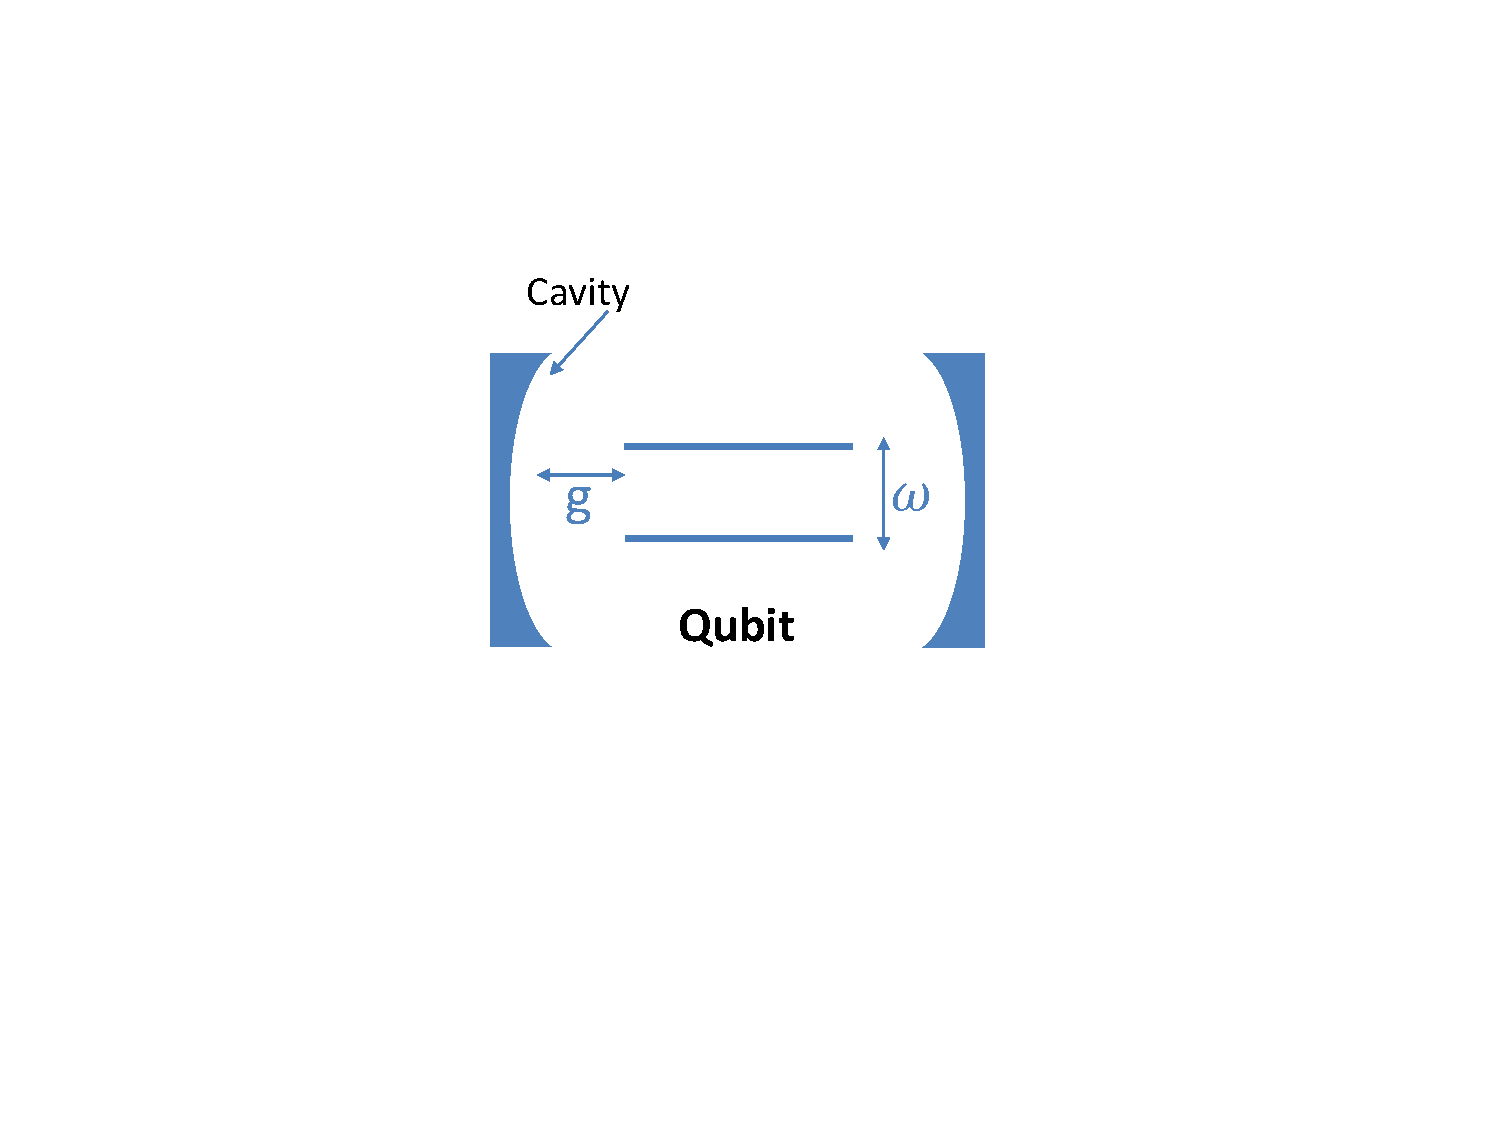
\includegraphics[width=0.5\textwidth]{Figr2a.pdf}
\caption{Single qubit in a perfect non leaky cavity}
\label{fig:Figr2a}
\end{figure}

Let the lower level be $\ket{g}$ and the upper level be $\ket{e}$. These two levels would be in contact with a electric field in the cavity. The cavity electric field in a quantized form is given by: 

%\begin{center}
\begin{align}\label{eq:3}
\hat { E } &=\hat{e}{ \left( \frac { \hslash \Omega  }{ { \epsilon  }_{ 0 }V }  \right)  }^{ { 1 }/{ 2 } }\left( {  a _{-} }+{  a  }_{ +  } \right) \sin { \left( kz \right) }
\end{align}
%\end{center}
%\textbf{cite gerry chp 2, 2.1}\\

The interaction Hamiltonian would be the following format effectively.
%\begin{center}
\begin{align}\label{eq:4}
{ H  }^{ \left( I \right)  }&= -\hat{D} {.} \hat{E}  \\
&=d g\left( {  a_{-}  }+{  a  }_{ +  } \right)
\end{align}
%\end{center}

where $ d $ = dipole moment operator of the atom, $\hat{D}$ is the dipole moment vector,%\\ 
%\textbf{cite gerry chp 4, 4.1}\\

%where
%\begin{center}
\begin{align}\label{eq:5}
g &= -{ \left( \frac { \hslash \Omega  }{ { \epsilon  }_{ 0 }V }  \right)  }^{ { 1 }/{ 2 } } \sin { \left( kz \right) }
\end{align}
%\end{center}

and  $ d = \hat{D}. \hat{e}$. At this point it is convenient to introduce the so-called atomic transition
operators.


%\begin{center}
\begin{align}\label{eq:7}
\sigma_{+}&=\dyad{e}{g},\quad \sigma_{-}= \dyad{g}{e}=\sigma_{+}^{ \dagger  },
\end{align}
%\end{center}\ket{e}\bra{g} \ket{g}\bra{e}
and the inversion operator 
%\begin{center}
\begin{align}\label{eq:8}
\sigma_{3}&=\dyad{e}-\dyad{g}.
\end{align}
%\end{center}\ket{g}\bra{g}
%$\bra{2} \ket{2} \braket{10} \dyad{e}{g}$
These operators obey the Pauli spin algebra
\begin{align}\label{eq:9}
[\sigma_{+},\thinspace\sigma_{-}] &=\sigma_{3}\\ %\notag
[\sigma_{3},\thinspace\sigma_{\pm}] &=2\sigma_{\pm}.
\end{align}

By parity, one can say that, the diagonal elements of ${d} = {0}$. Symmetry conditions coerce an atom to have a net zero dipole movement, if it is in an energy eigenstate. Hence the diagonal elements of ${d}$  would be zero $\expval{d}{e} = 0 = \expval{d}{g} $, 
%${d} = {0}$ This is also evident.

%\begin{center}
\begin{align}\label{eq:9.1}
\begin{split}
d&= d\dyad{g}{e}+{d}^{*}\dyad{e}{g}\\ 
&=d\sigma_{-} + d^{*}\sigma_{+} = d(\sigma_{+} + \sigma_{-}) 
\end{split}
\end{align}
%\end{center}\ket{g}\bra{e} \ket{e}\bra{g}
%d&= d\dyad{g}{e}+{d}^{*}\dyad{e}{g}\\ 
%&=d\sigma_{-} + d^{*}\sigma_{+} =d(\sigma_{+} + \sigma_{-}) \notag
where we have set $\mel{e}{d}{g}$ = d and have assumed, without loss of generality, that d is real. Thus the interaction Hamiltonian is %\eqref{eq:9.1}

%\begin{center}
\begin{align}\label{eq:10}
H^{(I)}&= \hslash\lambda(\sigma_{+} + \sigma_{-})({a}_{-} + {a}_{+})
\end{align}
%\end{center}
where $\lambda=dg/\hslash $%\newpage

\subsubsection{Derivation of the time dependence of the operators}
The explanation below closely follows that in chapter 2, section 2.1 of \citep{gerry2005introductory}.
The Hamiltonian of a harmonic oscillator is given by 
\begin{align}\label{eq:10.1}
H &=\hslash \Omega \left( { a}_{+  }a_{-} +\frac { 1 }{ 2 }  \right)
\end{align}
The Heisenberg equation for operators reads as
\begin{align}\label{eq:10.2}
\frac { d O  }{ dt } &=\frac { i }{ \hslash  } \left[ H ,O  \right] 
\end{align}

On substituting for the annihilation operator $a_{-}$ one gets
\begin{align}\label{eq:10.3} %\label{bch}
\frac { da_{-}  }{ dt } &=\frac { i }{ \hslash  } \left[ H ,a_{-}  \right]\notag\\
&=\frac { i }{ \hslash  }\left[\hslash \Omega \left( { a}_{+  }a_{-} +\frac { 1 }{ 2 }  \right),a_{-}\right]\\
&=i\Omega \left( { a}_{+  }a_{-}a_{-} -a_{-}{ a}_{+  }a_{-}  \right)\notag\\ 
&=i\Omega \left[{a}_{-},{{a}}_{+}\right]{a_{-}}=-i\Omega {a_{-}},\notag 
\end{align}

which has the solution
\begin{align}\label{eq:10.4}
{a}_{-}(t)&={a}_{-}(0){ e }^{ -i\Omega t }\\
{a}_{+}(t)&={a}_{+}(0){ e }^{  i\Omega t }
\end{align}

%\begin{align}

%\end{align}
Another way of doing it would be via the Baker-Hausdroff lemma \citep{sakurai1995modern}
For any two operators ${A} \thinspace $ and $\thinspace B,$

\begin{align}\label{eq:10.5}
{e }^{ i\lambda A  }B { e }^{ -i\lambda A }=B+{i}\lambda\left[A,B\right]+\frac{{\left(i\lambda  \right)}^{2}}{2!}\left[A\left[A,B\right]\right]+\dots
\end{align}

The solution to \eqref{eq:10.2} can be written as
\begin{align}\label{eq:10.6}
O(t)&={ e }^{ iH t/\hslash  }O (0){ e }^{ -iH t/\hslash  }
\end{align}


Applying it to \eqref{eq:10.6} with $a_{-}$ as $H$, $\lambda$ as $t/\hslash$ and  $B$ as $O (0)$ we get,
 \begin{align}\label{eq:10.7}
 O(t)&=O(0)+\frac { it }{ \hslash  } \left[ H ,O (0) \right]\notag \\ 
&+\frac { 1 }{ 2 !}\left(\frac { it }{ \hslash} \right)^{2}\left[H,\left[H,O(0)\right]\right]+......\notag\\
&+\frac { 1 }{ n !}\left(\frac { it }{ \hslash} \right)^{n}\left[H,\left[H,\left[H,....\left[H,O(0)\right]\right]\right]\right]+......
 \end{align}

Replacing $O$ by $a_{-}$ one obtains
\begin{align}\label{eq:10.8}
a_{-} (t)&=a_{-} (0)\left[ 1-i\Omega t-\frac { { \Omega  }^{ 2 }{ t }^{ 2 } }{ 2! } +i\frac { { \Omega  }^{ 3 }{ t }^{ 3 } }{ 3! } +........ \right] \notag \\
&=a_{-} (0){ e }^{ -i\Omega t }
\end{align}


%\newpage
Writing the evolution of operators once again,(just to avoid confusion)
%These can be derived by  either Baker Hausdorff lemma as shown in 
%\textbf{cite gerry chp 2, 2.1}   
%\begin{center}
%\end{center}
\begin{align}\label{eq:11}
a_{-}(t)&=a_{-}(0){e}^{-i{\Omega}t}\\ \notag 
a_{+}(t)&=a_{+}(0){e}^{i{\Omega}t}
\end{align}

Similarly,  the time evolution of the operators for the free-atomic case is as follows
\begin{align}\label{eq:12}
\sigma_{\pm}(t)&=\sigma_{\pm}(0){e}^{\pm{i}{\omega}t}
\end{align}
%\begin{center}
%\end{center}

expanding \eqref{eq:10} we have %equation ${2.11}$
\begin{align}\label{eq:13}
H^{(I)}&= \hslash\lambda(\sigma_{+} {a}_{-} + \sigma_{+}a_{+} + \sigma_{-} a_{-} + \sigma_{-}a_{+} )
\end{align}
%\begin{center}
%\end{center}

Let us look at approximate time dependencies for each of term in above mentioned equation. Using \eqref{eq:12} and \eqref{eq:11} one can compute the time dependence of each of the terms in the bracket in \eqref{eq:13}. Thus we can see that the approximate time dependences of the operator products
in ~\eqref{eq:13} are as follows:

%\begin{center}
\begin{align}\label{eq:14}
\sigma_{+}a_{-}\quad{\sim}\quad {e}^{i({\Omega}-{\omega})t}\\ 
\sigma_{+}a_{+}\quad{\sim}\quad {e}^{i({\omega}+{\Omega})t}\\
   \sigma_{-}a_{-}\quad{\sim}\quad {e}^{-i({\omega}+{\Omega})t}\\
\sigma_{-}a_{+}\quad{\sim}\quad {e}^{-i({\Omega}-{\omega})t} 
\end{align}
%\end{center}

If the electric field frequency  in the cavity is not quite detuned  from the spacing between the energy levels of the qubits then ${\Omega}$  is quite close to ${\omega}$. Hence  ${\omega} +  {\Omega} $ is very much larger than ${\omega} -  {\Omega} $ ( because ${\Omega} \approx  {\omega} $). On time averaging the Hamiltonian in \eqref{eq:13} the contribution of the middle two terms  becomes negligibly small if the above conditions hold. Since these terms oscillate very rapidly, on integration  they get multiplied with a pre-factor which is quite huge as compared to first two terms.  Hence they can be neglected. This approximation is also called as Rotating Wave Approximation (RWA). On carrying out RWA on \eqref{eq:13} it transforms to 


\begin{center}
\begin{align}\label{eq:15}
\hat{H}^{(I)}&= \hslash\lambda(\sigma_{+} a_{-}  + \sigma_{-}a_{+} )
%\hat{H}^{I} &=\hslash\lambda(\sigma_{+}  + \sigma_{-}a_{+})(\hat{a} + })
\end{align}
\end{center}


\section{Differential equation  governing time evolution}
\subsection{Closed vs.\ open quantum systems}
When one begins to learn quantum mechanics, it is implicitly assumed that all the systems that one studies exist in isolation. This is to say that they have no interaction with any other systems. In effect, all these system assumed to be closed and hence they are known as closed quantum systems. The system that we have here (i.e. two qubits in a leaky cavity ) dissipates energy into the environment. Thus it is an open system in contrast to  a closed one. %as opposed

\subsection{Need for density matrix formalism}
Let us consider any arbitrary Hamiltonian $H$. Being an operator it would satisfy its eigenvalue equation \footnote{The treatment in this and the following three sections somewhat follows that in \citep{traxler2009decoherence}}
\begin{align}\label{eq:17}
H\ket{m}&=E_{m}\ket{m}
\end{align}

%harmonic oscillator\\
Since the Hamiltonian is an energy operator the eigenvalues $E_{m}$  are the energies of the eigenstates\thinspace $\ket{m}$ 
\begin{align}\label{eq:18}
{ E }_{ m }&=\hslash \omega \left( m+\frac { 1 }{ 2 }  \right)
\end{align}
\begin{align}\label{eq:19}
H&=\frac { { p }^{ 2 } }{ 2m } +\frac { m{ \omega  }^{ 2 } }{ 2 } { x }^{ 2 }
\end{align}
The energy eigenbasis is just a common one in which the Hamiltonian is written. One can also write it in the position basis. (Infinite dimension here we come )
Just to have a feel of how different this representation is, let us calculate the probability $W(x)$ to find a particle in state $\ket{m}$ with energy $E_{m}$ at position $x$ is given by
\begin{align}\label{eq:20}
W(x)&=\vert \braket{x}{\thinspace m}\vert^{2}=|{ \varphi  }_{ m }\left( x \right) { | }^{ 2 }
\end{align}

To consider the most general case let us assume that the wave function is in the linear combination of energy eigenstates.  
\begin{align}\label{eq:21}
\ket{\psi}&=\sum _{ m=0 }^{ \infty  }{ { c }_{ m } }\ket{m}
\end{align}
This leads to 
\begin{align}\label{eq:22}
\psi{(x)}&=\braket{x}{\psi}\notag\\
&=\bra{x}\left(\sum _{ m=0 }^{ \infty  }{ { c }_{ m } }\ket{m}\right)\notag\\
&=\left(\sum _{ m=0 }^{ \infty  }{ { c }_{ m } }{\bra{x}}\ket{m}\right)\notag\\
&=\left(\sum _{ m=0 }^{ \infty  }{ { c }_{ m } }\bra{x}\ket{m}\right)\notag\\
&=\sum _{ m=0 }^{ \infty  }{ { c }_{ m } }{\varphi}_{m}{(x)}
 \end{align}

Using this let us again try to calculate $W(x)$ to find the particle at position $x$:

\begin{align}\label{eq:23}
W{(x)}&=\vert\braket{x}{\psi}\vert^{2}=\vert{\psi}(x)\vert^{2}\notag\\
&={\varphi}^{*}{(x)}\varphi{(x)}\notag\\
&=\left(\sum _{ m=0 }^{ \infty  }{ { c }_{ m }^{ * } } { \varphi  }_{ m }^{ * }\left( x \right)\right)\left(\sum _{ n=0 }^{ \infty  }{ { c }_{ n } } { \varphi  }_{ n }\left( x \right)\right)\notag\\
&=\sum _{ m,n }^{  }{ { c }_{ m }^{ * } } { c }_{ n }{ \varphi  }_{ m }^{ * }\left( x \right){ \varphi  }_{ n }\left( x \right)
\end{align}

Partitioning the sum in two parts, one in which the the indices are equal and one which they are not. 
\begin{align}\label{eq:24}
W(x)&=\sum _{ m=0 }^{ \infty  }\vert{ { c }_{ m }\vert^{2} }{\vert\varphi}_{m}\vert^{2}+ \sum _{ m\neq n }^{  }{ { c }_{ m }^{ * } } { c }_{ n }{ \varphi  }_{ m }^{ * }\left( x \right){ \varphi  }_{ n }\left( x \right)\notag\\
&=\sum _{ m=0 }^{ \infty  }\vert{ {c } _{ m }\vert^{2} }{W}_{m}+ \sum _{ m\neq n }^{  }{ { c }_{ m }^{ * } } { c }_{ n }{ \varphi  }_{ m }^{ * }\left( x \right){ \varphi  }_{ n }\left( x \right)\notag\\
&=\sum _{ m=0 }^{ \infty  }{p}_{m}{W}_{m}(x) + \sum _{ m\neq n }^{  }{ { c }_{ m }^{ * } } { c }_{ n }{ \varphi  }_{ m }^{ * }\left( x \right){ \varphi  }_{ n }\left( x \right)
\end{align}

Where $\vert{{c}_{m}\vert^{2}}={p}_{m}$ is the probability to find the particle in ${m}^{th}$ energy-eigenstate with the features ${0}\le{p}_{m}\le{1}$ and ${\sum _{ m}{p}_{m} =1}$ and\thinspace ${W}_{m}={\vert\varphi}_{m}\vert^{2}$ is the probability to find the ${m}^{th}$ energy-eigenstate position ${x}$.

\begin{align}\label{eq:25}
&=\sum _{ m=0 }^{ \infty  }{p}_{m}{W}_{m}{(x)}+ \sum _{ m\neq n }^{  }{ { c }_{ m }^{ * } } { c }_{ n }{ \varphi  }_{ m }^{ * }\left( x \right){ \varphi  }_{ n }\left( x \right)
\end{align}

\begin{align}\label{eq:26}
\sum _{ m=0 }^{ \infty  }+ \sum _{ m\neq n }^{  }  
\end{align}

The first part $\sum_{m=0}^{\infty }$ is the sum of the probabilities of finding the particle in the $m^{th}$ eigenstate times the probability to find the  $m^{th}$ eigenstate at position $(x)$.


The second part $\sum _{m\neq 0}$ is the double sum of the off diagonal terms.
The second part is what it imparts "quantumness" to quantum.
\subsubsection{Digression}
From \cite{churchill1990complex} any complex number can be expressed as either:
\begin{enumerate}
\item x+i{y} $ ( x, y \in \mathds{R})$ 
\item r $e^{i\theta} ( r, \theta \in \mathds{R})$
\end{enumerate}
%\textnormal{where }
where: 
\begin{itemize}
\item x = real part
\item y = imaginary part of the complex no 
\item r = modulus of the complex no 
\item $\theta$ = argument  of the complex no or phases in physics and engineering . 
\end{itemize}

For the sake of convenience, let us choose the $2^{nd}$ representation. Therefore one can write the expansion coefficients (of the wave function $\ket{\psi}) \quad c_{m}$ as

\begin{align}\label{eq:27.1}
{ c }_{ m } &=\sqrt { { p }_{m}}{ e }^{ i{ \alpha  }_{ m } }\notag\\
{ c }_{ m }^{*} &=\sqrt { { p }_{m}}{ e }^{ i{ \alpha  }_{ m } }
\end{align}
where ${ c}_{ m }$ is complex number, ${ { p }_{ m } }$ is real number and ${ \alpha  }_{ m }$ is an arbitrary phase. 
%\left({\alpha}_{m}\right)
%For expansion coefficient ${ c }_{ m }\left( { \alpha  }_{ m } \right)$ 
%original equation 
%\begin{align}\label{eq:27}
%{ c }_{ m }\left( { \alpha  }_{ m } \right) &=\sqrt { { p }_{ m } } { e }^{ i{ \alpha  }_{ m } }
%\end{align}
\par
${c}_{m}$ is a function of ${{p}_{m}}$ , ${\alpha}_{m}$. Let us say we have partial information about the state $\ket{\psi}$. If one knows ${c}_{m}$ fully one can uniquely determine $\ket{\psi}$. In real life, one rarely has complete information about anything. One usually has to make do with what one has.
Therefore it would not be right to assume that one has complete knowledge about the state $\ket{\psi}$. This implies, by virtue of what we had stated earlier that our knowledge of $c_{m}$ too, is imperfect. This leads to the following possibilities: 

\begin{itemize}
\item $\lbrace{{p}_{m}}\rbrace$ is not known 
\item $\lbrace{\alpha}_{m}\rbrace$ is not known
\item we have partial knowledge of both $\lbrace{{p}_{m}}\rbrace$,  $\lbrace{\alpha}_{m}\rbrace$
\end{itemize}
\par
For reasons of pedagogy, time, space, etc. let us go ahead with option 2 i.e  we have no idea about $\lbrace{\alpha}_{m}\rbrace$. Since we don't know $\lbrace{\alpha}_{m}\rbrace$ all the quantities we can measure are those in which any dependence over $\lbrace{\alpha}_{m}\rbrace$ is averaged away. To put it in another way any quantity that one calculates say z $({p}_{m}, {\alpha}_{m})$ we would have to find  ${\left\langle{z}\right\rangle}_{\alpha_{m}}$ (or equivalently ${\left\langle{z}\right\rangle}_{phase}$ owing to our incomplete information.

An interesting thing to note in this connection is that 

%Averaging over all phases 

\begin{align}\label{eq:28}
\left\langle{ e }^{ i{ \alpha  }_{ m } }\right\rangle &=\frac { 1 }{ 2\pi  } \int _{ 0 }^{ 2\pi  }{ { e }^{ i{ \alpha  }_{ m } } } { d }{ \alpha  }_{ m } =0
\end{align}


%From the standard mathematics (one can see this by using the euler identity and integrating separately the real and imaginary parts or its discrete analog)  

\subsubsection{coming back to \eqref{eq:24} we have}
\begin{align}\label{eq:29}
W{(x)}&=\sum _{ m }^{\infty  }{ { p }_{m}}{W}_{ m }\left( x \right)+\sum _{ m\neq{n}} c_{m}^{*}\thinspace c_{n}{ \varphi  }_{ m }^{ * }(x){ \varphi  }_{ n }(x)\notag\\
W{(x)}&=\sum _{ m }^{\infty  }{ { p }_{m}}{W}_{ m }\left( x \right)+\sum _{ m\neq{n}}\sqrt{{p}_{m}} e^{-i{\alpha}_{m}} \sqrt{{p}_{n}} e^{i{\alpha}_{n}} { \varphi  }_{ m }^{ * }(x){ \varphi  }_{ n }(x)\notag\\
W{(x)}&=\sum _{ m }^{\infty  }{ { p }_{m}}{W}_{ m }\left( x \right)+\sum _{ n\neq m }^{  }{ \sqrt { { p }_{ m } }  } \sqrt{{p}_{n}} { e }^{ i({ \alpha  }_{ m }-{ \alpha  }_{ n }) }{ \varphi  }_{ m }^{ * }(x){ \varphi  }_{ n }(x)
\end{align}

%considering the probability $W{(x)}:$ Equation:11

%\begin{align}
%W{(x)}=\sum _{ m }^{  }{ { p }_{ m } } |{ \psi  }_{ m }\left( x \right) { | }^{ 2 }+\sum _{ n\neq m }^{  }{ \sqrt { { p }_{ m } }  } \sqrt{{p}_{n}} { e }^{ i({ \alpha  }_{ n }-{ \alpha  }_{ m }) }{ \varphi  }_{ m }^{ * }(x){ \varphi  }_{ n }(x)\notag
%\end{align}

On averaging we get:
\begin{align}\label{eq:30}
\left\langle {W}{(x)}\right\rangle _{phase} &=\sum _{m=0}^{ \infty  }{ { p }_{ m }{ W }_{ m } } (x)\\
&=\sum _{ m=0 }^{ \infty  }{ \left| { c }_{ m } \right|^{2} \left| { \varphi  }_{ m } \right|^{2}  }\notag\\
&=\sum _{ m=0 }^{ \infty  }{ \left| { c }_{ m } \right|^{2} \left| { \varphi  }_{ m }(x) \right|^{2}  }\notag
\end{align}

One can also go about getting $W(x)$ in an other way.
Starting from \eqref{eq:20}

\begin{align}\label{wrong:1}
W(x) &= \vert\braket{x}{\psi}\vert^{2}\\
\bigg\langle {{W}(x)}\bigg\rangle_{phase} 
&=\bigg\langle \vert\braket{x}{\psi}\vert^{2}\bigg\rangle_{phase}\notag\\
&=\bigg\langle\vert\bra{x}\thinspace\ket{\psi}\vert^{2}\bigg\rangle_{phase}\notag\\
&=\vert\bra{x}\bigg\langle{\ket{\psi}}\bigg\rangle \vert^{2}_{phase}\notag
\end{align}

\begin{align}\label{eq:31}
\left\langle{\ket{\psi}}\right\rangle_{phase}&=\frac{1}{2\pi}\int_{0}^{2\pi}\ket{\psi}{d{\alpha}_{m}}\notag\\
&=\frac{1}{2\pi}\int_{0}^{2\pi}\sum _{m}\sqrt{{p}_{m}} e^{-i{\alpha}_{m}}\ket{m}{d{\alpha}_{m}}\notag\\
&=\frac{1}{2\pi}\sum _{m}\sqrt{{p}_{m}}\Bigg(\int_{0}^{2\pi} e^{-i{\alpha}_{m}}\ket{m}{d{\alpha}_{m}}\Bigg)\ket{m}\notag\\
&=\frac{1}{2\pi}\sum _{m}\sqrt{{p}_{m}} \times  (0) \times  \ket{m}\notag\\
&=0
\end{align}
\begin{align}\label{eq:32}
\therefore W(x)&=\Biggl|\bra{x}\bigg\langle{\ket{\psi}}\bigg\rangle\Biggr|^{2}_{phase}\notag \\
&= 0 
\end{align}

\textbf{= a contradiction with \eqref{eq:30} }.
Therefore this doesn't seem to be right. Some thing is wrong somewhere.
Lets go back to \eqref{eq:20} and start again.
We had 
\begin{align}\label{eq:33}
W(x) &= \vert\braket{x}{\psi}\vert^{2}\notag\\
&=\braket{x}{\psi} \braket{x}{\psi}\notag\\
&=\braket{x}{\psi} \braket{\psi}{x}\notag\\
&=\bra{x}\thinspace\ket{\psi}\bra{\psi}\thinspace\ket{x}
\end{align}
this can also be written as 
\begin{align}\label{aft33:1}
&\bra{x}\underbrace{\dyad{{\psi}}}\ket{x}
\end{align}
where the quantity in the under brace
\begin{align}\label{aft33:2}
\bra{x} \thinspace {\rho} \ket{x}
\end{align}

is known as the density matrix. It is denoted by symbol $\rho$. Whenever one has incomplete information it is better to work with density matrix.
Let us expand this quantity in terms of position basis
\begin{align}\label{aft33:3}
\rho= \dyad{\psi}&=\Biggl(\sum_{m} {c}_{m}\ket{m}  \Biggr)\Biggl(\sum_{n} {c}_{n}\ket{n} \Biggr)^{\dagger}\notag\\
&=\Biggl(\sum_{m} {c}_{m}\ket{m}  \Biggr)\Biggl(\sum_{n} ({c}_{n}\ket{n})^{\dagger} \Biggr)\notag\\
&=\Biggl(\sum_{m} {c}_{m}\ket{m}  \Biggr)\Biggl(\sum_{n} \ket{n}^{\dagger}{c}_{n}^{\dagger} \Biggr)\notag\\
&=\Biggl(\sum_{m} {c}_{m}\ket{m}  \Biggr)\Biggl(\sum_{n} \bra{n}{c}_{n}^{*} \Biggr)\notag\\
&=\sum_{m}{c}_{m}\ket{m}\sum_{n}\bra{n}{c}_{n}^{*}\notag\\
&=\sum_{m}\sum_{n}{c}_{m}\ket{m}\bra{n}{c}_{n}^{*}\\
&=\sum_{m}\sum_{n}{c}_{m}{c}_{n}^{*}\ket{m}\bra{n}%\notag\\
\end{align}

Substituting from \eqref{eq:27.1}  we get %modify equation : 9

\begin{align}\label{aft33:4}
&=\sum_{m}\sum_{n}\sqrt{{p}_{m}} e^{i{\alpha}_{m}} \sqrt{{p}_{n}} e^{-i{\alpha}_{n}}\dyad{m}{n}\notag\\
&=\sum_{m}\sum_{n}\sqrt{{p}_{m}}  \sqrt{{p}_{n}} e^{i{\alpha}_{m}} e^{-i{\alpha}_{n}}\dyad{m}{n}\notag\\
&=\sum_{m}\sum_{n}\sqrt{{p}_{m}}\sqrt{{p}_{n}} e^{i(\alpha_{m}-\alpha_{n})} \dyad{m}{n}
\end{align}
One can also write it as
\begin{align}\label{aft33:5}
\rho &=\sum_{m}{p}_{m}\dyad{m}{m}+\sum _{ n\neq m }^{  }\sqrt { { p }_{ m }{ p }_{ n } }  { e }^{ i({ \alpha  }_{ m }-{ \alpha  }_{ n }) }\dyad{m}{n}
\end{align}

Averaging over all phases 
\begin{align}\label{aft33:6}
\left\langle{p}\right\rangle _{phase} & = \sum_{m} {\rho}_{m}\dyad{m}{m} = \sum_{m} {\rho}_{mm}\dyad{m}{m}
\end{align}
Using all this information in \eqref{aft33:2}
% Rearranging above equation 
\begin{align}\label{aft33:7}
\left\langle{W}(x)\right\rangle _{phase} &= \left\langle\expval{\rho}{x}\right\rangle_{phase}\\
&=\bra{x}\left\langle{\rho}\right\rangle_{phase}\ket{x}\\
&=\bra{x}\left(\sum_{m} {p}_{m}\dyad{m}{m}\right) \ket{x}\\
&=\sum_{m} {p}_{m}\bra{x}\left(\dyad{m}{m}\right) \ket{x}\notag\\
&=\sum_{m} {p}_{m}\braket{x}{m} \braket{m}{x}\notag\\
&=\sum_{m} {p}_{m}\braket{x}{m} \braket{x}{m}\notag\\
&=\sum_{m} {p}_{m}\vert\braket{x}{m}\vert^{2}\notag\\
&=\sum_{m} {p}_{m} W_{m}{(x)}
\end{align}
Which is the correct answer \eqref{eq:30} unlike \eqref{wrong:1}\\
Any density matrix is defined by (since information about phase is usually unknown)

\begin{align}
\rho &= \sum p_{m}\dyad{m}\\
\vert c_{m}\vert^{2}&=p_{m}=1 
\end{align}

\subsection{Properties of Density matrices}
%\citep{traxler2009decoherence}
\subsubsection{Positivity}

\begin{align}\label{aft33:8}
\rho \geq 0
\end{align}
Explanation : \\
Given any $\ket{v}\expval{\rho}{v} \geq {0}$\\
The only condition is that $\ket{v}$ should not be  a null vector. \\


Differently expressed\\ 
\begin{align}\label{aft33:9}
\expval{\rho}{\varphi}&=\bra{\varphi}{\sum_{m}p_{m}}\dyad{m}\ket{\varphi}\notag\\
&={\sum_{m}p_{m}}\bra{\varphi}\dyad{m}\ket{\varphi}\notag\\
&={\sum_{m}p_{m}}\vert\braket{\varphi}{m}\vert^{2}\geq{0}
\end{align}

\subsubsection{Self Adjoint}
\begin{align}
{\rho }={\rho}^{\dagger}
\end{align}

The Adjoint of an operator $ A = \dyad{\varphi}{\psi}$ is \\
\begin{center}
$ A^{\dagger} =\left( \dyad{\varphi}{\psi}\right)^{\dagger}$
$=\left(\bra{\psi}\right)^{\dagger} \left(\ket{\varphi}\right)^{\dagger} = \ket{\psi} \bra{\varphi} = \dyad{\psi}{\varphi}$
\end{center}
\begin{align}\label{aft33:10}
\rho^{\dagger} &= \bigg(\sum_{m}p_{m}\dyad{m}\bigg)^{\dagger}\\
&= \sum_{m}\big(p_{m}\dyad{m}\big)^{\dagger}\\
&= \sum_{m}\left(\dyad{m}\right)^{\dagger}p_{m}^{\dagger}\\
&= \sum_{m}\left(\dyad{m}\right)^{\dagger}p_{m}^{*}\\
&= \sum_{m}p_{m}^{*}\left(\dyad{m}\right)^{\dagger}\\
&= \sum_{m}p_{m}\left(\dyad{m}\right)^{\dagger}
\end{align}

$\big(\because p_{m} \in \mathds{R}$ \big) since it is a probability 

\begin{align}
&=\sum_{m}p_{m}\left(\dyad{m}\right)^{\dagger}
\end{align}


%\\&=\braket{\varphi}{\psi} \braket{\psi}{\varphi}
%Commonly the adjoint ${D}^{\dagger}$ of an operator $D=\dyad{\varphi}{\psi}$ is defined by ${D}^{\dagger}=\left(\dyad{\varphi}{\psi}\right)^{\dagger}=\dyad{\psi}{\varphi}$, which gives for ${\rho}: {\rho}^{\dagger}=\dyad{\psi}{\psi}^{\dagger} = \dyad{\psi}{\psi}={\rho}$


\subsubsection{Unit trace}

\begin{align}
tr({\rho})= 1
\end{align}

The trace of an operator $A$ is as follows 

\begin{align}\label{aft33:11}
tr{(A)} &=\sum_{i}\expval{A}{i} \\ 
\therefore tr{(\rho)} &=\sum_{i}\expval{\rho}{i} \\
 &=\sum_{i}\bra{i}\bigg(\sum_{m}p_{m}\dyad{m}\bigg) \ket{i}  \\
 &=\sum_{i}p_{m}\braket{i}{m} \braket{m}{i}\\
 &=\sum_{i}p_{i} = 1
\end{align}
$\because$ sum of all probabilities add to $1$

\begin{align}\label{aft33:12}
\rho^{2}&={\rho}\\
\rho^{2}&={\rho}\times{\rho}\\
&= \bigg(\sum_{m}p_{m}\dyad{m}\bigg) \bigg(\sum_{n}p_{n}\dyad{n}\bigg)\\
&=\sum_{m}\sum_{n} p_{m}p_{n}\dyad{m}\dyad{n}\\
&=\sum_{m}\sum_{n} p_{m}p_{n} \ket{m} \delta_{mn} \bra{n}\\
&=\sum_{m}\sum_{n} p_{m}p_{n}\delta_{mn} \dyad{m}{n}\\
&=\sum_{n}p_{n}p_{n}\dyad{n}\\
&=\sum_{n}p_{n}^{2}\dyad{n}
\end{align}
$\sum_{n}p_{n}^{2}\dyad{n} \neq \rho$ in general.\\
If $p_{n} = 1 $ for $n=1$ and $p_{n} = 0$ otherwise\\
then $\rho^{2} = \dyad{1}$ and $\rho = \dyad{1}$....
 $\therefore \rho^{2} = \rho$\\
If $p_{n} = 1$ then the density $\rho$ is a pure state otherwise it is a mixed state.

\subsubsection{expectation value}
The expectation value of an operator ${A}$ is given as
\begin{align}\label{aft33:13}
\left\langle{A}\right\rangle &= \expval{A}{\psi}\\
tr(\rho{A}) &=\sum_{i} \expval{\rho{A}}{i}\\
&=\sum_{i} \bra{i} \bigg(\sum_{m}p_{m}\dyad{m} {A}\bigg)\ket{i}\\
&=\sum_{i} \sum_{m}p_{m} \braket{i}{m} \matrixel{m}{A}{i}\\
&=\sum_{i} \sum_{m}p_{m}\thinspace\delta_{im} \matrixel{m}{A}{i}\\
&=\sum_{m}p_{m}\expval{A}{m}\\
&=\sum_{m}\vert{c}_{m}\vert^{2}\expval{A}{m}\\
&=\sum_{m} {c}_{m} {c}_{m}^{*} \expval{A}{m}\\
&=\sum_{m} \expval{{c}_{m}^{*} {A} {c}_{m}}{m}\\
&=\bigg(\sum_{m}\bra{m}{c}_{m}^{*}\bigg) A \bigg(\sum_{m}{c}_{m}\ket{m}\bigg)\\
&=\expval{A}{\psi}=\left\langle{A}\right\rangle\\
&\therefore tr(\rho{A}) =\left\langle{A}\right\rangle
\end{align}

\subsection{Equation of Motion for density matrix}   
From Schroedinger's equation one has
\begin{align}\label{aft33:23}
i\hslash \frac { \partial  }{ \partial t } \ket{\psi_{i}}&=H\ket{\psi_{i}}
\end{align}
Taking the complex conjugate we get 
\begin{align}
-i\hslash \frac { \partial  }{ \partial t } \bra{\psi_{i}}&=\bra{\psi_{i}}H
\end{align}

Applying  this equation for the density matrix  we obtain:

\begin{align}\label{aft33:24}
i\hslash \frac { \partial  }{ \partial t }\rho&=i\hslash\sum_{i}{p}_{i}\left(\dyad{\dot { \psi_{i}  }}{\psi_{i}} + \dyad{\psi_{i}}{\dot { \psi_{i}  }} \right)\notag\\
&=\sum_{i}{p}_{i}\left(H\dyad{{ \psi_{i}  }}{\psi_{i}} - \dyad{\psi_{i}}{{ \psi_{i}  }}H \right)\notag\\
&=H{\rho} - {\rho}H
\end{align}

Thus we obtain the  Von Neumann-equation: 

\begin{align}\label{aft33:25}
i\hslash \frac { \partial  }{ \partial t }\rho &=\left[H,\rho\right]
\end{align}

\subsection{A prelude to Lindblad  master equation}
The universe is always composed of our system of interest
$S$ and the environment $E$ that it is in. Considering the total Hilbert space we get:
\begin{align}\label{aft33:42}
\mathcal{H} &= \mathcal{H}_{S}\thinspace \otimes\thinspace \mathcal{H}_{E}
\end{align}
The general form of Hamiltonian is:
\begin{align}\label{aft33:43}
H(t)&=H_{S}\thinspace \otimes\thinspace\mathbb{1}_{E} + \mathbb{1}_{S}\thinspace \otimes\thinspace H_{E}+ H_{I} (t) 
\end{align}

where $H_{S}$ is the Hamiltonian of the open system, $H_{E}$ is the Hamiltonian of the environment and $H_{I} (t)$ denotes the interaction between system and environment.
The operators which act exclusively  on the system $S$ are of the form 

\begin{center}
$A\thinspace \otimes\thinspace\mathbb{1}_{E} \quad with \quad A \thinspace  \epsilon \thinspace \mathcal{H}_{S}$
\end{center}

We obtain  density matrix of the system ${S}$ by tracing over the  environment. The expectation value of $A$ is represented by:
\begin{align}\label{aft33:44}
\rho^{S} &= tr_{E}(\rho)\\
\left\langle {A}\right\rangle &=tr_{S}(\rho^{S} {A}) 
\end{align}

Since the universe is a closed system it evolves unitary with time with the unitary responsible for it given by:
\begin{align}\label{aft33:45}
U\left( t,{ t }_{ 0 } \right) &=T{ e }^{ -i\int _{ { t }_{ 0 } }^{ t }{ H\left( t \right) dt }  }
\end{align}

Subjecting the universe density matrix to partial trace over the environment we get.  
\begin{align}\label{lowsleep:1}
\rho^{S}(t)&=tr_{E}\thinspace\left( U(t,t_{0})\thinspace \rho\thinspace (t_{0})\thinspace U^{\dagger}(t,t_{0})\right)
\end{align}

Writing down the Von Neumann equation for a closed system we have:$(\hslash=1)$
\[\frac { \partial}{ \partial t }\rho(t)=-i\left[H(t),\rho(t)\right], .\]

As explained before let us take a trace over the environment again

\begin{align}\label{aft33:46}
\frac { \partial}{ \partial t }\rho^{S}(t) &= -i \thinspace tr_{E}
\left( \left[H(t),\rho(t)\right] \right)
\end{align}

\subsubsection{Dynamical map, Operator sum representation, quantum dynamical semi-groups}

Let us assume absence of initial correlations between the system and the environment. Hence  the density operator can be described by a tensor product of $\rho^{S}$ and $\rho^{E}$:
\begin{align}\label{aft33:47}
\rho(0) &=\rho^{S}(0)\thinspace \otimes\thinspace \rho^{E}\\
\rho^{S}(0)&\rightarrow\rho^{S}(t)=V(t)\thinspace\rho^{S}(0)\equiv t{r}_{E }U(t,0)\thinspace{\rho}^{S}(0)\otimes { \rho}^{E}{U}^{t}(t,0)
\end{align}

(where $V (t): \mathcal{H}_{S} \rightarrow \mathcal{H}_{E} $ is called dynamical map.) (In the coming sections we will show that a dynamical map $V (t)$ can be completely characterized by operators acting on $\mathcal{H}_{S}.$) Writing down the spectral decomposition of $\rho^{E}$:
\begin{align}
\rho^{E} &= \sum_{k}p_{k}\thinspace\dyad{\phi_{k}}{\phi_{k}} 
\end{align}

where $ 0\leq {{p}_{k}} \thinspace and \thinspace \sum p_{k} =1$.


Schematic diagram of the time evolution is as follows.
\begin{gather}
\rho(0) =\rho^{S}(0)\thinspace \otimes\thinspace \rho^{E} \rightarrow\frac{U(t,0)}{unitary\thinspace time-evolution}\rho(t)= U(t,0)\thinspace {\rho}^{S}(0)\otimes{\rho}^{E}{U}^{\dagger}(t,0)\label{aft33:48}\\
\downarrow t{ r }_{ E }\notag \\
\rho^{S}(0) \rightarrow\frac{V(t)}{dynamical\thinspace map}\rho^{S}(t) = V(t)\thinspace \rho^{S}(0)\label{aft33:50}
\end{gather}






For the density matrix  of the universe we arrange for the following:
\begin{itemize}
\item at beginning $t = 0$ the density matrix is given as a product state:
\end{itemize}
\begin{align}\label{aft33:51}
\rho(0) &= \rho^{S}(0)\thinspace \otimes\thinspace \rho^{E}
\end{align}
\begin{itemize}
\item at $t = 0$ the environment represents a pure state - it  simplifies the discussions to a great extent
\end{itemize}
\begin{align}
\rho^{E}(0)&=\dyad{\phi_{0}}{\phi_{0}}
\end{align}
%\newpage
Going back to \eqref{lowsleep:1} and making use of above inputs we have 

\begin{gather}
\rho_{tot}\rightarrow U\rho^{S}(0)\thinspace \otimes\thinspace \rho^{E}U^{\dagger}\label{aft33:52}\\
\Downarrow \notag\\
\rho^{S}=tr_{E}\rho \rightarrow \sum_{k} \bra{\phi_{k}}U\rho^{S}(0)\thinspace \otimes\thinspace \dyad{\phi_{0}}{\phi_{0}}U^{\dagger}\ket{\phi_{k}}\label{aft33:54}
\end{gather}








(where $\lbrace\ket{\phi_{k}}\rbrace$ denote the complete states of the environment.)\\ 
Introducing  Kraus - operators which live in the $\mathcal{H_{S}}$ Hilbert space
\begin{align}\label{aft33:55}
W_{K}&=\colon\bra{\phi_{k}}U\ket{\phi_{0}}\\
{W}_{k}^{ \dagger} &=\colon \bra{\phi_{0}}U^{\dagger}\ket{\phi_{k}}
\end{align}
with the property
\begin{align}\label{aft33:56}
\sum_{k}{ W }_{ k }^{ \dagger}{ W }_{ k } &=\sum_{k}\bra{\phi_{0}}U^{\dagger}\ket{\phi_{k}}\bra{\phi_{k}}U\ket{\phi_{0}}=\expval{U^{\dagger}U}{{\phi_{0}}}=\expval{\mathbb{1}_{S+E}}{{\phi_{0}}}={\mathbb{1}_{S}}
\end{align}

Thus the dynamical map of the time evolution of the density matrix of the system can be representation in terms of a sum of Kraus-operators:
\begin{align}
\rho^{S}(0) &\rightarrow\sum_{k}W_{k}\thinspace\rho^{S}(0)W_{k}^{\dagger}= V\left[\rho^{S}(0)\right]=\rho^{S}(t)
\end{align}

\subsubsection{Properties of the dynamical map $V (t)$:}
\begin{itemize}
\item The dynamical map V (t) is trace conserving.
\begin{align}\label{aft33:57}
tr_{S}\left(\rho^{S}(t)\right) 
&=tr_{S}\left(V\rho^{S}\right)\notag \\
&=tr_{S}\left(\sum_{k}W_{k}\thinspace\rho^{S}(0)W_{k}^{\dagger} \right)\notag \\
&=\sum_{k} tr_{S}\left(W_{k}\thinspace\rho^{S}(0)W_{k}^{\dagger} \right)\notag \\
&=\sum_{k} tr_{S} \left(W_{k}^{\dagger} W_{k}\thinspace\rho^{S}(0)\right)\notag  \because \textnormal{cyclicity of trace}\\
&=tr_{S} \left(\sum_{k} W_{k}^{\dagger} W_{k}\thinspace\rho^{S}(0)\right)\notag \\
&=tr_{S} \left( \left(\sum_{k} W_{k}^{\dagger} W_{k} \right)\thinspace\rho^{S}(0)\right)\notag \\
&=tr_{S} \bigg( \mathbb{1} \thinspace \rho(0) \bigg)\thickspace  from \thickspace \eqref{aft33:56}\notag \\
&=tr_{S}\left(\rho^{S}(0)\right)
\end{align}

\item $V (t)$ is a convex linear map.
\begin{align}\label{aft33:58}
V(t)\sum_{i}p_{i}\thinspace\rho_{i} &=\sum_{i}p_{i}V(t)\thinspace\rho_{i}, \\
\sum_{i}p_{i}&=1 \rightarrow \textnormal{ convex sum}
\end{align}
\item The dynamical map V (t) is completely positive.
\end{itemize}
\begin{align}\label{aft33:59}
V(t)\otimes { 1 }_{ n }\ge 0 \thinspace &\textnormal \thinspace {\mathcal{H}  }_{ S }\otimes \mathds{C}^{n}
\end{align}

Let be a map $V(t)[\rho] \geq 0$ for all $\rho \geq 0$ and for all $t \geq 0$ on a finite dimensional complex 
Hilbert space. Then the map $V$ is {\it completely positive} if the extension

\begin{align}\label{aft33:60}
V_{n}(t) &=V(t)\otimes \mathbb{1}_{n}\\ 
V_{n}(t)\left[\rho\otimes\omega\right] &=V(t)\left[\rho\right]\otimes\omega\geq{0}
\end{align}

for all $\rho\thinspace \epsilon \thinspace \mathcal{H}$ and for all $\omega \thinspace \epsilon \thinspace \mathds{C}^{n}$

\subsubsection{$V (t)$ is completely positive ,$\Leftrightarrow$ $V (t)\otimes V (t) \geq 0 $ is positive.} 
This theorem is important for entangled systems, a counter example to complete positivity is the partial transposition.
\par 
\subsubsection{Markovianity}
If one  assumes that the characteristic time scale of the environment $\tau_{E}$ is several orders of magnitude less than that of the system $\tau_{S}$ whatever excitations quantum information transferred to the environment is lost.
quite fast as compared to the same process occurring in the system. 
The characteristic time scales are determined by some correlation functions proportional to $e^{-\frac{t} {\tau_{E}}}$ in case of the environment and $e^{-\frac{t}{\tau_{S}}}$ in case of the system.


This enables  the dynamical map $V$ to form a semi group:

\begin{align}\label{aft33:61}
V(t_{1})V(t_{2}) &=V\left(t_{1}+t_{2}\right) \thinspace where\thinspace  t_{1},t_{2}\geq{0}
\end{align}
The semi-group can be written in terms of its generators as :
\begin{gather}
V(t) =e^{\mathcal{L}\thinspace{t}}\label{aft33:62}\\
\Downarrow\notag \\
\rho^{S}(t) = V(t)\rho^{S}(0)=e^{\mathcal{L}\thinspace {t}}\rho^{S}(0)\label{aft33:63}
\end{gather}
The generator satisfies  so-called master equation
\begin{align}\label{aft33:64}
\frac{\partial}{\partial{t}} \rho^{S}(t) &= \mathcal{L}\thinspace \rho^{S}\thinspace(t)
\end{align}

where $\mathcal{L}$ is the so-called Liouville-operator.


\subsection{Lindblad master equation}

The aim of this section is to  construct the most general form of the Liouville equation for a -finite dimensional complex Hilbert-space $\mathcal{H}_{s} $ with dim $\mathcal{H}_{s} = N^{2}$. our approach begins with constructing out of Kraus-operators an equation which contains the Hamilton-operator (plus remaining operators).
This method goes back to \cite{lindblad1976}  and to \cite{gorini1976completely} 




The master equation due to Lindblad is given by:

\begin{align}\label{aft33:99}
\frac { d }{ dt } { \rho  }^{ S }(t)=-\frac { i }{ \hslash  } \left[ H,{ \rho  }^{ S }(t) \right] -D\left[ { \rho  }^{ S }(t) \right] 
\end{align}

where ${\rho  }^{ S }$ is the density matrix of the system and $D\left[ { \rho  }^{ S } \right]$ is the so-called dissipator

\begin{align}\label{aft33:100}
D[{ \rho  }^{ S }]=\frac {1}{2}\sum_{k=1}^{ {N}^{2}-1}{{\lambda}_{k}}\left({A}_{k}^{ \dagger}{ A }_{ k }{ \rho  }^{ S }+{ \rho  }^{ S }{ A }_{ k }^{ \dagger  }{ A }_{ k }-2{ A }_{ k }\thinspace{ \rho  }^{ S }{ A }_{ k }^{ \dagger  } \right) 
\end{align}

\begin{align}\label{aft33:101}
D[{ \rho  }^{ S }]=\frac { 1 }{ 2 } \sum _{ k}{ { \lambda  }_{ k } } \left(\left[ { A }_{ k }^{ \dagger  },{ A }_{ k }{ \rho  }^{ S }\right]+\left[{ \rho  }^{ S }{ A }_{ k }^{ \dagger  },{ A }_{ k }\right] \right) 
\end{align}

with the Lindblad-operators $A_{k}$ and the (positive) decoherence constants ${\lambda}_{k} \geq {0}$ which
are a quantitative measure for decoherence.

Assuming a weak coupling limit between the system and the environment

\begin{align}\label{aft33:102}
H\equiv H_{S+E}&=H_{S} + H_{E}+H_{int}
\end{align}
for $ H_{E}, H_{int}\rightarrow 0 \Rightarrow H= H_{S}$\\

\subsubsection{Proof of the Lindblad-master-equation} 

Consider the dynamical map for the time-evolution of the density matrix of the system:

\begin{align}\label{aft33:103}
{ \rho  }^{ S }\rightarrow V\left[ { \rho  }^{ S } \right]&=\sum _{k}{{W}_{k}}{\rho}^{S}{W}_{k}^{\dagger  }\\
W_{k}&=\matrixel{\phi_{k}}{U}{\phi_{0}}
\end{align}

With the unitary operator $U =e^{-\frac{i}{h}Ht}$ and the property $\sum_{k}{W}_{k}^{\dagger}{W}_{k}=1$\\

The dynamical map fulfills the following properties:

\begin{itemize}
\item trace conserving
\item convex linear
\item completely positive
\end{itemize}
Some assumptions:

\begin{itemize}
\item The characteristic time scale of the system $\delta{t}$ is much smaller than the lifetime of the system $\tau_{S}$:
\begin{center}
$\delta{t}\ll \thinspace \tau_{S}$
\end{center}
\item The environment should "forget" about the system, this is a so-called Markov process:
\begin{center}
$\tau_{E}\ll \thinspace\delta{t} $
\end{center}
\end{itemize}
Restarting from \eqref{aft33:103} keeping in mind the above assumptions taking into account.:

\begin{align}\label{aft33:104}
\rho^{S}(\delta{t})&=V\left[ { \rho  }^{ S }(0) \right] =\sum _{ k }W_{k}{ { \rho  }^{ S } } (0){ W }_{ k }^{ \dagger }={ \rho  }^{ S }(0)+\mathcal{O}(\delta{t})
\end{align}

We see that the first Kraus-operator is of the order $\sim {1}_{S}+\mathcal{O}(\delta{t})$, while all other Kraus-operators $\sim \mathcal{O}(\delta{t})$. are of the order of$(\delta{t})$ 

\begin{align}\label{aft33:105}
W_{0}&={\mathbb{1}_{S}} +\left(K-\frac{i}{\hslash}H\right)\delta{t}\\
W_{k}&=A_{k}\sqrt[]{\delta{t}}
\end{align}

where $K$ and $H$ are hermitian operators and $A_{k}$ is the Lindblad operator. From the normalization condition \eqref{aft33:56} we get:
\begin{gather}
\sum_{k}W_{k}^{\dagger}W_{k}=\mathbb{1}_{S}+\left(2K+\sum_{k}A_{k}^{\dagger}A_{k}\right)\delta{t}+\mathcal{O}(\delta{t}^{2})\label{aft33:106}\\
\Downarrow\notag \\
K=-\frac{1}{2}\sum A_{k}^{\dagger}A_{k}\label{aft33:107}
\end{gather}

Plugging the value of K back into \eqref{aft33:104}  we get 

\begin{align}\label{aft33:108}
\rho^{S}(\delta{t})&=W_{0}{ { \rho  }^{ S } }{ W }_{0}^{ \dagger } +\sum W_{k}{ { \rho  }^{ S } } (0){ W }_{ k }^{ \dagger }=\notag\\
&=\left(\mathbb{1}_{S}+\left(K-\frac{i}{\hslash}H\right)\delta{t}\right)\rho^{S}(0) \left(\mathbb{1}_{S}+\left(K+\frac{i}{\hslash}H\right)\delta{t}\right)+\delta{t}\sum_{k}{A}_{k}\rho^{S}(0){A}_{k}^{\dagger}=
\end{align}

Neglecting all higher order terms, we are left with
\begin{align}\label{aft33:109}
&=\rho^{S}(0)+\delta{t} \lbrace-\frac{i}{\hslash} \left[H,\rho^{S}(0)\right]-\frac{1}{2}\left(\sum A_{k}^{\dagger}A_{k}\thinspace\rho^{S}(0)+\rho^{S}(0)A_{k}^{\dagger}A_{k}-2A_{k}\thinspace\rho^{S}(0)A_{k}^{\dagger} \right)\rbrace
\end{align}
\begin{center}
$\Downarrow $
\end{center}
\begin{align}\label{aft33:110}
\lim _{\delta t\rightarrow 0 }{\frac{{\rho}^{S}\left(\delta t \right)-{\rho}^{S}\left(0\right)}{\delta t}} &=\frac{d}{dt}{\rho}^{S}(t)\vert_{t=0}&=-\frac{i}{\hslash} \left[H,\rho^{S}(t)\right]\vert_{t=0}-D\left[\rho^{S}(t)\right]\vert_{t=0}
\end{align}
Note:
Here we have derived  at $t = 0$ but it holds for any time and we have rescaled ${A}_{k}=\sqrt{{\lambda}_{k}} {A}_{k}$


%%


%%% Local Variables: 
%%% mode: latex
%%% TeX-master: "../mainrep"
%%% End: 

\chapter{System Description and Previous work}
\section{Description of System}
\subsection{Parts of the system}
\subsubsection{Qubits}
A qubit is a quantum bit, the analog in quantum computing to the binary digit or bit of classical computing. Just as a bit is the basic unit of information in a classical computer, a qubit is the basic unit of information in a quantum computer. \citep{Whatisqubit} 
%\textbf{cite whatis}
\par
In simple words, a qubit is a two level quantum mechanical system.
%\newline \textbf{\emph{fig3}}
\begin{figure}[h]
\centering
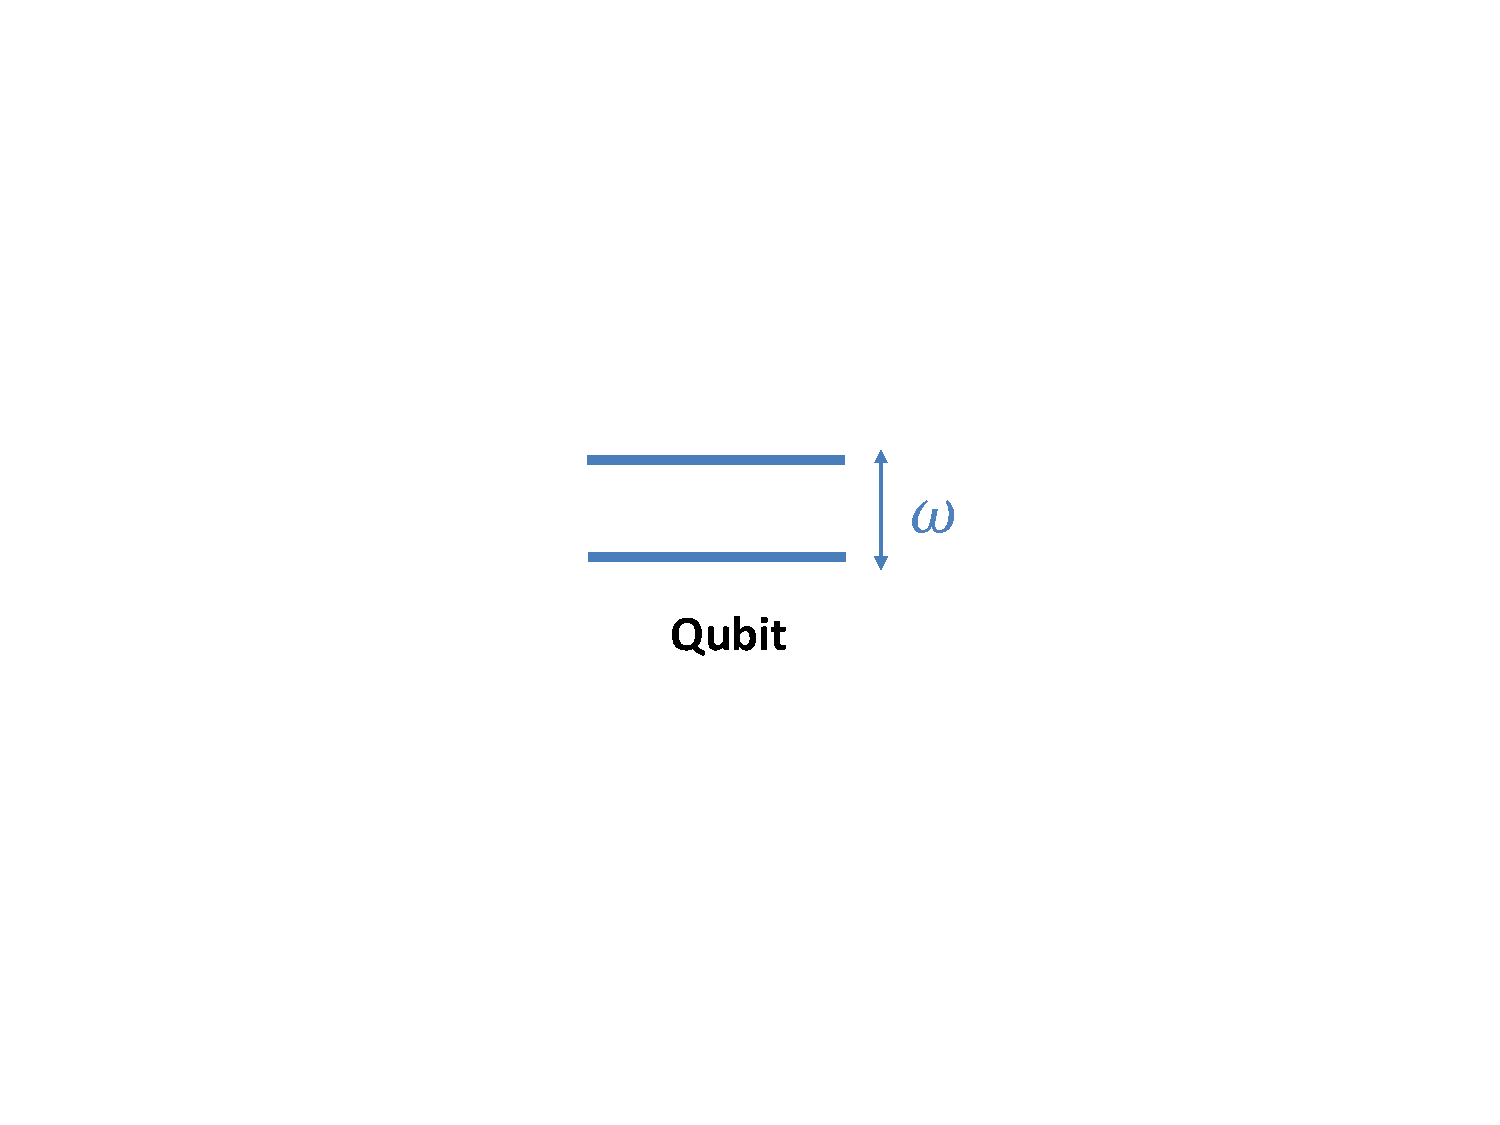
\includegraphics[width=0.5\textwidth]{Figr3a.pdf}
\caption{Qubit}
\label{fig:Figr3a}
\end{figure}


\subsubsection{Electromagnetic cavity}
An electromagnetic cavity  is an enclosure where standing electromagnetic waves can be sustained for considerable periods of time with or without an external driving field.%\citep{wiki:resonator}
%\textbf{ cite wiki resonator}
%\newline \emph{fig4}
\begin{figure}%[h]
\centering
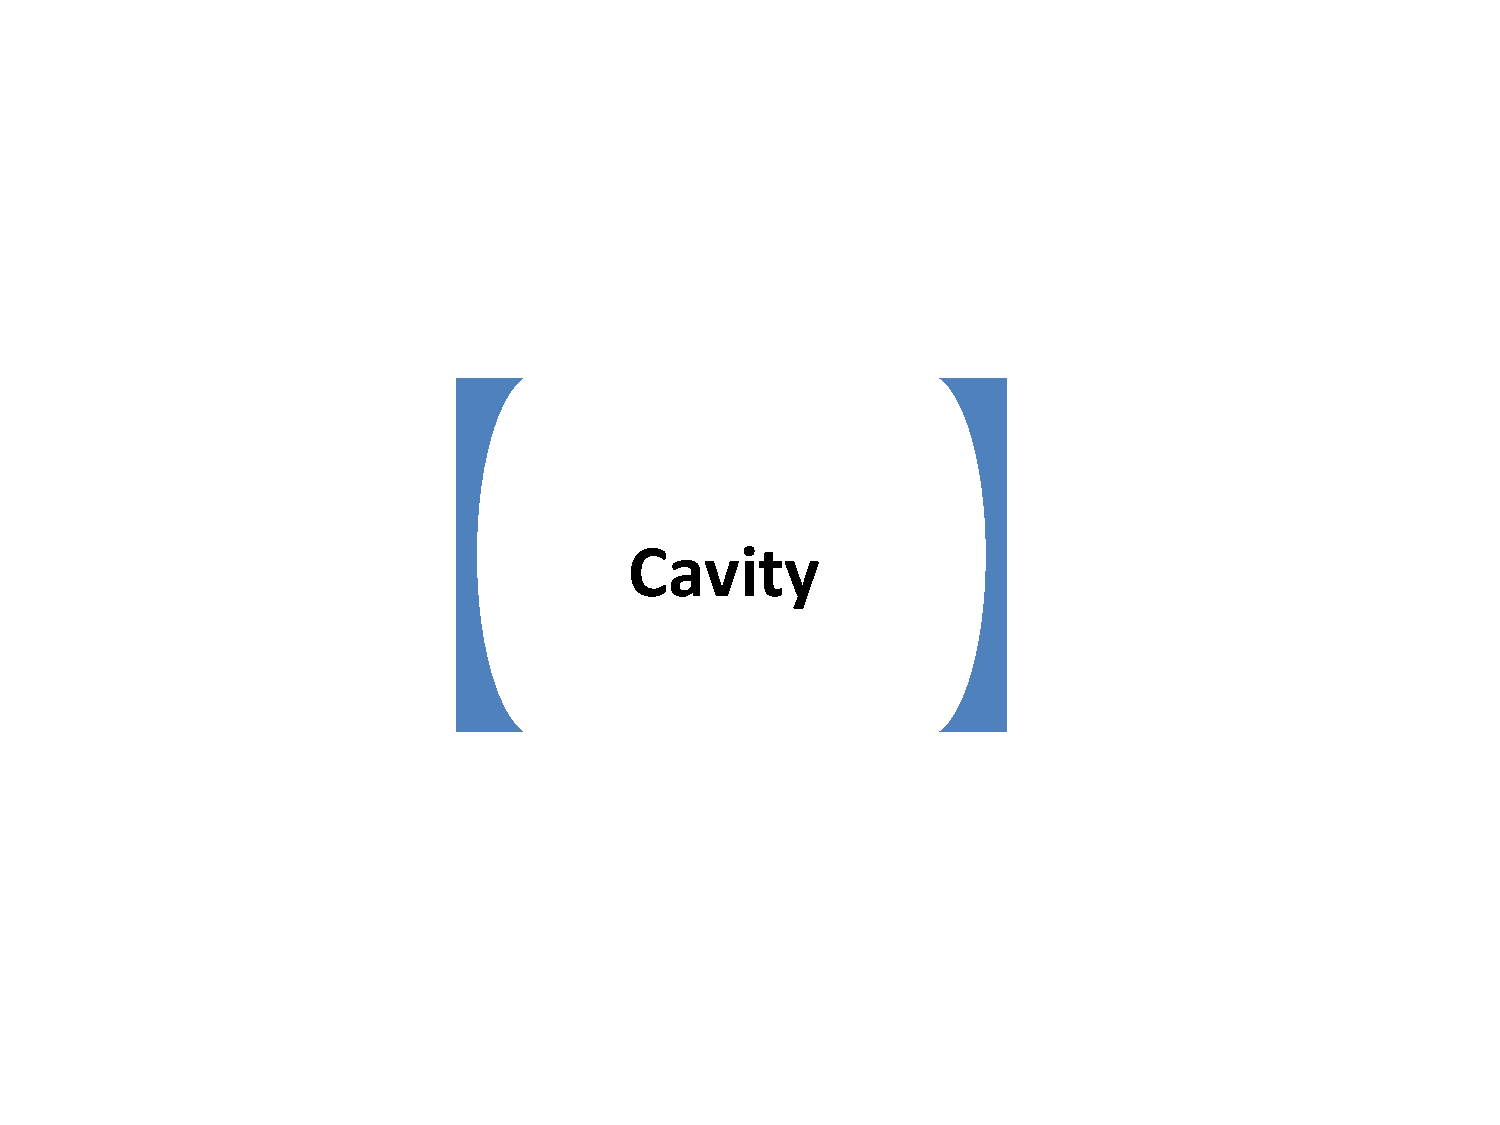
\includegraphics[width=0.5\textwidth]{Figr4a.pdf}
\caption{Cavity}
\label{fig:Figr4a}
\end{figure}

\subsubsection{Physics of system}
To exemplify how state transfer could be enhanced by tweaking the underlying Hamiltonian it would be better to do so by means of trying it out on an actual physical system. The physical system \citep{Tejas_APS1}  that we choose for this purpose is as follows : 
\begin{figure}[!h]
\centering
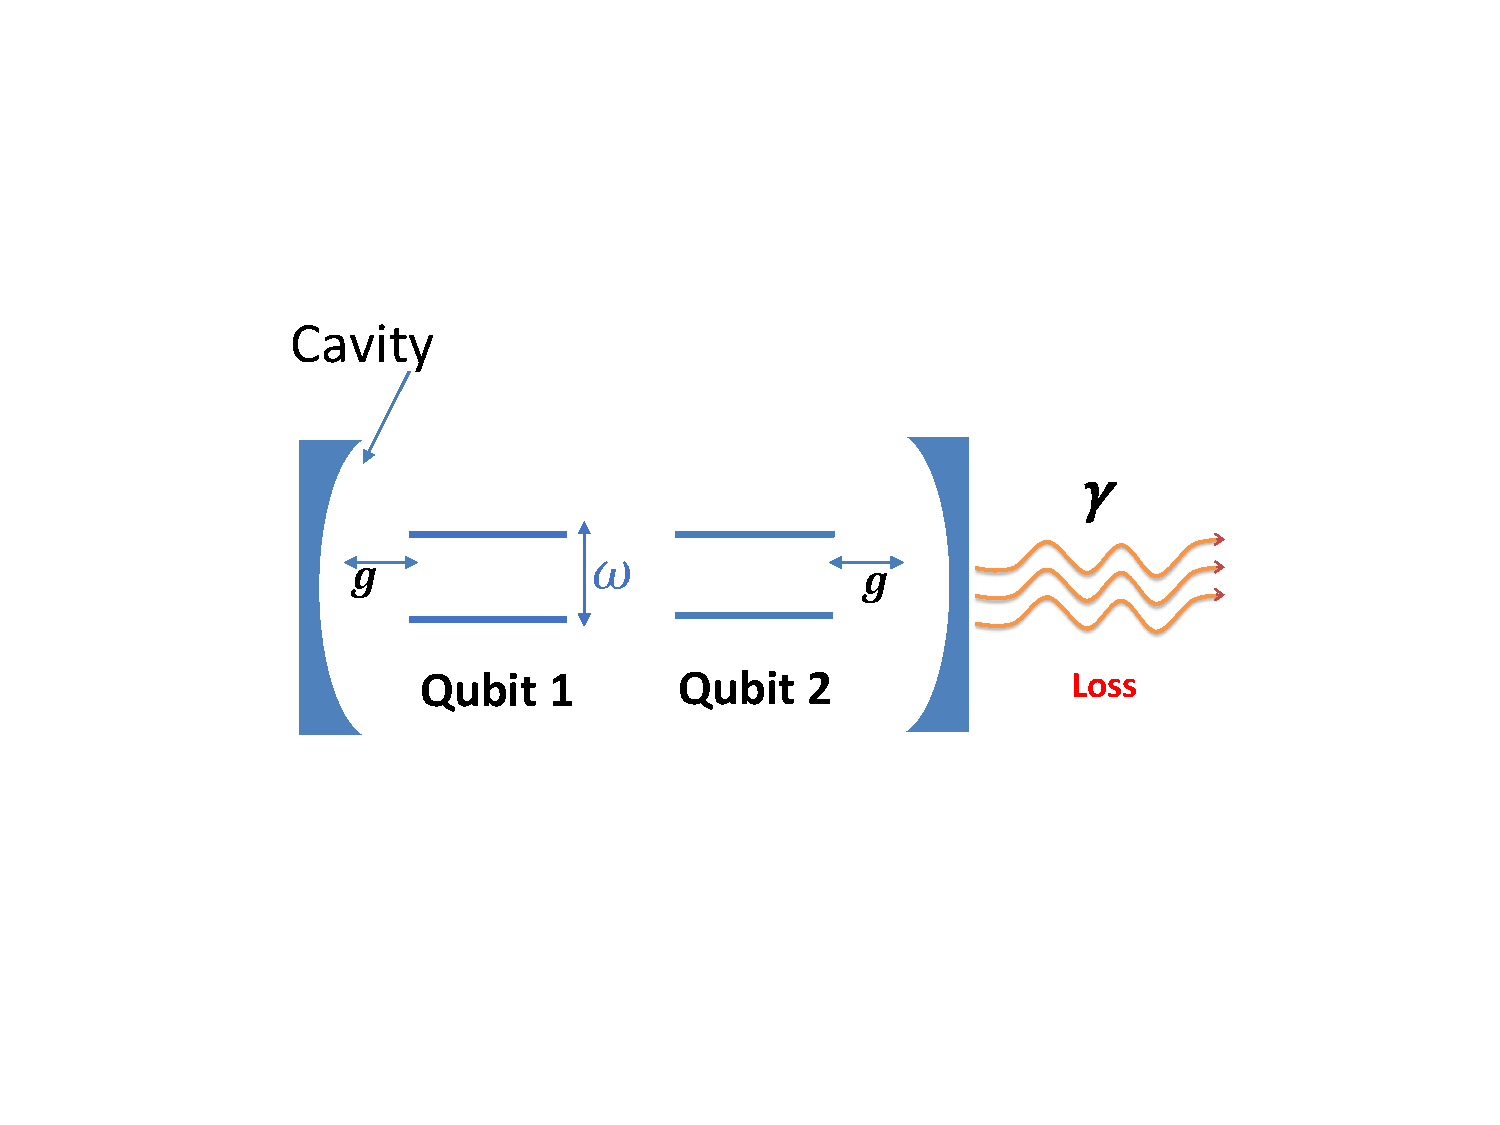
\includegraphics[width=0.8 \textwidth]{Figr1a.pdf}
\caption{Two qubits in a leaky cavity}
\label{fig:Figr1a}
\end{figure}


%The statement of the problem is as follows:
\begin{itemize}
\item We have:%\textbf{ cite my old aps }
\begin{enumerate}
\item Two qubits each with an energy difference of $(\hslash\thinspace{\omega})$.
\item A single mode lossy cavity approximated as a harmonic oscillator with energy spacing of $(\hslash\thinspace{\Omega})$.  
\end{enumerate}
\item Dissipation of quantum information occurs at a characteristic rate ($\gamma$).
\item There is no interaction between the qubits themselves.
\item Both the qubits are coupled to the cavity
\item The only way the qubits can communicate with each other is via the cavity
\end{itemize}

\subsection{Hamiltonian of the system}
The Hamiltonian of the system can be written as follows:
\begin{align}\label{eq:1}
H &= H_{0} + V
\end{align}
where $H_{0}$ is the bare Hamiltonian and $V$ is the coupling Hamiltonian. 
The bare Hamiltonian can be written as
\begin{align}\label{eq:2}
{H}_{0}&=\frac{\omega}{2}\thinspace{\sigma}_{z}\thinspace\otimes I^{(2)}\otimes{I^{(n)}}\thinspace + \thinspace\frac{\omega}{2}\thinspace{I^{(2)}}\thinspace\otimes\thinspace{\sigma}_{z}\otimes{I^{(n)}}\thinspace+\thinspace\Omega\thinspace I^{(2)}\otimes I^{(2)}\otimes{a}_{+}{a}_{- }
\end{align}
Where: 
\begin{itemize}
\item $\omega$ = frequency corresponding to the energy spacing  between the two levels of each qubit.
\item $\Omega$ = frequency corresponding to the difference in the energy levels of the cavity.
\item ${\sigma}_{z}, {\sigma}_{+}, {\sigma}_{-}$ =  Pauli matrices.   
\item ${a}_{+}, {a}_{-}$ = creation and annihilation operators for the cavity.
\item $I^{(2)}$ is the identity in the qubit Hilbert space.
\item $I^{(n)}$ is the identity in the harmonic oscillator Hilbert space.
\item $\hbar$ is set to be equal to $1$ in accordance with the usual practice. 
\end{itemize}
In the above equation~\eqref{eq:2} %\textbf{From2.2 }
\begin{itemize}
\item The first part represents bare Hamiltonian for the qubit 1.
\item The second part represents that of qubit 2.
\item The third  part represents that of  cavity. 
\end{itemize}

Now we will talk about how one would write down the interaction Hamiltonian $V$. Since, our system consists of qubits in a cavity effectively we have a double Jaynes Cummings type of Hamiltonian 
In our case since we have two qubits  we will have two couplings, \(g_{1}\) and \(g_{2}\). ${g}_{1}$ is the parameter related to the  strength of the coupling between the first qubit and the cavity. Similarly for ${g}_{2}$. So, following the discussion in the previous chapter we have 
\begin{align}\label{eq:15.1}
V &= V_{1} + V_{2}
\end{align}
Where: 
\begin{align}\label{eq 15.2}
V_{1}&= g_{1}\left({\sigma  }_{ - }\otimes I^{(2)}\otimes { a }_{ + }\thinspace + \thinspace{ \sigma }_{+}\otimes I^{(2)}\otimes{a}_{ - }\right)\\
V_{2}&= g_{ 2 }\left(I^{(2)}\otimes { \sigma  }_{ - }\otimes { a }_{ + }+I^{(2)}\otimes { \sigma  }_{ + }\otimes { a }_{ - }\right)
\end{align}


%\begin{itemize}
%\item $V_{1}= g_{1}\left({\sigma  }_{ - }\otimes I^{(2)}\otimes { a }_{ + }\thinspace + \thinspace{ \sigma }_{+}\otimes I^{(2)}\otimes{a}_{ - }\right)$
%\item $V_{2}= g_{ 2 }\left(I^{(2)}\otimes { \sigma  }_{ - }\otimes { a }_{ + }+I^{(2)}\otimes { \sigma  }_{ + }\otimes { a }_{ - }\right)$
%\end{itemize}

Putting all this together we get equation 
\begin{equation}\label{eq:16}
V= g_{1}\left({\sigma  }_{ - }\otimes I^{(2)}\otimes { a }_{ + }\thinspace + \thinspace{ \sigma }_{+}\otimes I^{(2)}\otimes{a}_{ - }\right)\thinspace
+\thinspace g_{ 2 }\left(I^{(2)}\otimes { \sigma  }_{ - }\otimes { a }_{ + }+I^{(2)}\otimes { \sigma  }_{ + }\otimes { a }_{ - }\right)
\end{equation}
Thus the full Hamiltonian is as follows:
\begin{multline}\label{FullH:1}
H =\frac{\omega}{2}\thinspace{\sigma}_{z}\thinspace\otimes I^{(2)}\otimes{I^{(n)}}\thinspace +\thinspace\frac{\omega}{2}\thinspace{I^{(2)}}\thinspace\otimes\thinspace{\sigma}_{z}\otimes{I^{(n)}}\thinspace+\thinspace\Omega\thinspace I^{(2)}\otimes I^{(2)}\otimes{a}_{+}{a}_{- } \\
+ g_{1}\left({\sigma  }_{ - }\otimes I^{(2)}\otimes { a }_{ + }\thinspace + \thinspace{ \sigma }_{+}\otimes I^{(2)}\otimes{a}_{ - }\right)\thinspace
+\thinspace g_{ 2 }\left(I^{(2)}\otimes { \sigma  }_{ - }\otimes { a }_{ + }+I^{(2)}\otimes { \sigma  }_{ + }\otimes { a }_{ - }\right)
\end{multline}
Where all the symbols are as defined earlier and $\hbar$ is set to be equal to $1$ in accordance with the usual practice.  
\subsubsection{Working of the system } 
This system works as follows:
\begin{itemize}
\item Qubit 1 is coupled to the cavity via the coupling Hamiltonian ${g}_{1}({\sigma  }_{ - }\otimes I^{(2)}\otimes { a }_{ + }\thinspace + \thinspace{ \sigma }_{+}\otimes I^{(2)}\otimes{a}_{ - })$. Through these coupling the state of qubit 1 is  being transferred to the cavity.
\item Similar to qubit 1, qubit 2 is also coupled via the coupling Hamiltonian ${g}_{2}\left(I^{(2)}\otimes { \sigma  }_{ - }\otimes { a }_{ + }+I^{(2)}\otimes { \sigma  }_{ + }\otimes { a }_{ - }\right)$. Through this coupling the information from the cavity is being transferred to qubit 2.
\item All this while the cavity is also leaking quantum information at a rate $\gamma$.
\end{itemize}

\subsection{Choice of Lindbladian operator}

Having derived the Lindblad equation in the previous chapter it is time to decide what would be the Lindbladian operators. One thing that we know is they must be of the same dimensions, shape etc. as that of the density matrix. This is because both of them live in the Hilbert space of the system.
\par 
We know that the cavity is a leaky one i.e. it undergoes spontaneous emissions. The cavity has been modelled as a harmonic oscillator. On undergoing emission the oscillator drops down from one fock state to the one below it. This is equivalent to the action of a annihilation operator acting on the harmonic space oscillator.
\par
Thus we can write 

\begin{align}\label{eq:1001}
L = I^{(2)} \otimes I^{(2)} \otimes {a}_{-}
\end{align}

where all the terms are the same as defined before 

\subsection{Putting it all together}
After all this hard work we end up with,

\begin{equation}\label{eq:1002}
\frac { {d\rho}_{s}}{dt} = -{ i\thinspace } [{ H },\thinspace { \rho  }_{ s }] +\gamma \left({ { L }\thinspace{ \rho}_{ s } }\thinspace { L }^{ \dagger  }-\frac { 1 }{ 2 } \{ { L }^{ \dagger}\thinspace{L},{\rho  }_{ s }\}\right)
\end{equation}

Where:
\begin{itemize}
\item $\rho_{s}$ = Density matrix for the system which includes both the qubits and the cavity.
\item  Total Hamiltonian as written in \eqref{FullH:1}\begin{multline}\notag
H =\frac{\omega}{2}\thinspace{\sigma}_{z}\thinspace\otimes I^{(2)}\otimes{I^{(n)}}\thinspace +\thinspace\frac{\omega}{2}\thinspace{I^{(2)}}\thinspace\otimes\thinspace{\sigma}_{z}\otimes{I^{(n)}}\thinspace+\thinspace\Omega\thinspace I^{(2)}\otimes I^{(2)}\otimes{a}_{+}{a}_{- } \\
+ g \left({\sigma  }_{ - }\otimes I^{(2)}\otimes { a }_{ + } + { \sigma }_{+}\otimes I^{(2)}\otimes{a}_{ - }
+ I^{(2)}\otimes { \sigma  }_{ - }\otimes { a }_{ + }+I^{(2)}\otimes { \sigma  }_{ + }\otimes { a }_{ - }\right)
\end{multline} where we have additionally set $g_{1}$ equal to $g_{2}$ and replaced both of them by $g$, since this is the case which we could consider while performing the numerical calculations. Here $g$ is the common coupling strength of the qubits to the cavity.
\item $ {L} = I^{(2)} \otimes I^{(2)} \otimes {a}_{-} $  Lindbladian operator as in \eqref{eq:1001}
\item $\gamma$ = Characteristic rate of dissipation for the cavity. 
\item $\hbar$ is set to be equal to $1$ in accordance with the usual practice. 
\end{itemize}


\section{Previous work}
The question that we wish to answer is that could we improve the state transfer by varying the coupling constant $g$ with time. In short, our aim is to see if one could enhance the fidelity to the target state if we make the coupling constant time dependent.   We tried to answer these questions by writing a code  in MATLAB \textsuperscript{\textregistered}.  This code uses the built in function fmincon (an interior point algorithm which minimizes functions using some gradient optimization techniques).
One may wonder why  use fmincon if one wants to maximize ? Doesn't fmincon contain the word "min" instead of "max". The trick is that we minimize the negative of the fidelity to determine the optimum pulse sequence for a piece wise constant $g(t)$.

In this chapter we present some of the results that we obtained by numerically solving the Lindblad equation \Eqref{eq:1002} in MATLAB\textsuperscript{\textregistered}.

We have undertaken a comparative study of how the fidelity changes as a function of the strength of the coupling $g$, (we take both the couplings $g_{1}$ and $g_{2}$ to be equal to $g$). \textbf{We consider two cases one in which the  $g$ is a constant w.r.t. time and other in which  $g$ is a function of time.}

In the case where the coupling strength $g$ is constant with respect to time we plot the graph of fidelity versus the constant value of coupling strength $g$. This is known as the static case. 

For the case of the time dependent $g$ we plot the graph as a function of the maximum value of coupling strength $g_{max}$ allowed to the system. This is said to be the dynamic case.

The parameters of the system under study are:
\begin{itemize}
\item $\omega = 1 s^{-1} $ (frequency corresponding to the energy spacing between the two levels of each qubit)
\item $\Omega = 1 s^{-1} $ (frequency corresponding to the difference in energy levels of the cavity).
\item $\gamma = 1 s^{-1} $ (characteristic rate of dissipation for the cavity) 
\item $t_{max} = 16 s^{-1}$ (time for which the system is allowed to evolve)
\end{itemize}

As one can see value of $\Delta = \omega - \Omega = 0 $. Here $\Delta$ is the detuning parameter. We have considered the simple case of $\Delta = {0}$ so that we can have almost perfect transfer of quantum state information between the qubit and cavity. There is almost no interaction between the qubits themselves. The only way the qubits could communicate with each other is via the cavity. The time is chosen so as to allow at least one Rabi oscillation of within the given evolution time. This is done to allow the qubits enough time to interact with the system. 

\begin{align}
Q_{a}&=\begin{pmatrix} 0.5 & 0.5 \\ 0.5 & 0.5 \end{pmatrix}\\
Q_{b} &= \begin{pmatrix} 0 & 0 \\ 0 & 1 \end{pmatrix}\\
\alpha &= 0.01{i}
\end{align}

We will write the state of the system as
\begin{center}
qubit\textsubscript{1} state  $\otimes$  qubit\textsubscript{2} state \thinspace $\otimes$ cavity  state 
\end{center}
The initial state of the system is 
\begin{align}
Q_{a} \otimes Q_{b} \otimes \dyad {\alpha} 
\end{align}
(where $\ket{\alpha}$ is a coherent state). 
The final state of the system is 
\begin{align}
Q_{b} \otimes Q_{a} \otimes \dyad {\alpha} 
\end{align}

As one would soon realise we are trying to implement the swap gate for the two qubits. 
The fidelity metric that we use is:
\begin{align}
fidelity(A,B) = \bigg|\sqrt {tr\left( A B \right) + 2 \sqrt { det\left( A \right) det\left( B \right)}}\thinspace \bigg|
\end{align}
The fidelity between the target and the initial state is $0.5$. Therefore the initial fidelity is 0.5. This is the approximate starting point in every graph involving fidelity. The time step for numerical calculations is $0.01{s}$ 



On referring to \Figref{A_fidelity_static_g__semilog_large_range} and \Figref{H-fk_fidelity_static_g__semilog_large_range_-_Final} we see that for both the static as well as the dynamic case the fidelity rises initially up to a certain value and then starts dropping after remaining at its maximum value for some range of $g$. %a\textsuperscript{2} a\textsubscript{5}

%\begin{table}[h]
%\begin{tabular}{|l|c|c|c|}
%\hline
%       &\textbf{Peak occurs at\textsuperscript{*} (g 
%       value)}    & \textbf{Peak value\textsuperscript{*}  (Fidelity)}     &\textbf{Descent begins at\textsuperscript{*} (g 
%       value)} \\      \hline
% Static    &0.2             &0.8      &1  \\     \hline
% Dynamic   &0.5            &0.96      &1.75  \\     \hline
%\end{tabular}
%\end{table}

%* rough value\\

In the range from ${10}^{-20}\left(\sim 0\right)$ to ${10 }^{-1}$ the fidelity stays put  at approximately 0.5. It  is evident from \Figref{A_fidelity_static_g__semilog_large_range} and \Figref{H-fk_fidelity_static_g__semilog_large_range_-_Final} there seems to be almost no activity between 0 and 0.1 after which a sharp rise takes place. 

 In this range the ratio of the coupling strength $g$ to the dissipation rate $\gamma$ is less than one \[\frac {g}{\gamma}<1\]

The fidelity at $t=0$ is 0.5 as stated earlier. Since the coupling strength $g$ is low as compared to $\gamma = 1$, there is almost no interaction between the qubits and the cavity. Hence the system remains nearly at the initial state even though time passes. So there is no difference between the static and dynamic case. 

When the coupling strength $g$ is of the same order of magnitude as $\gamma$ the dissipation rate $\gamma$ $({g}\sim{\gamma}=1)$ the state transfer between the qubits and the cavity occurs to some extent. This occurs sufficiently faster than the speed at which dissipation occurs (at a rate determined by $\gamma=1$) due to the leaky nature of the cavity. Hence the state transfer between the qubits is partially successful. In the static case the fidelity obtained is less than or equal to that in the dynamic case. This is because at each step in time the optimizer chooses a value of the coupling constant which  would maximize the final fidelity function. This fidelity is calculated in the following steps: 


\begin{enumerate}
\item We have $\frac {{d\rho}_{s}}{dt} = -{i} [{ H },\thinspace { \rho  }_{ s }] +\gamma \left({ { L }\thinspace{ \rho}_{ s } }\thinspace { L }^{ \dagger  }-\frac { 1 }{ 2 } \{ { L }^{ \dagger}\thinspace{L},{\rho  }_{ s }\}\right)$. Here $g$ (i.e. the coupling strength ) is function of time.
\item We can integrate this to give $\rho\left({t,g{(t)}}\right)$ if  $g{(t)} $ is known.
\item We can then calculate the fidelity between $\rho\left({t,g{(t)}}\right)$ and $\rho_{final}$. Thus we get fidelity $f\left({t,g{(t)}}\right)$ as a function of time $t$ and $g{(t)}$
\item The function which gives fidelity at the final time $t_{max}$ is $f'\left(t_{max}, g{(t)}\right)$
\item We can optimize this function $f'\left(t_{max}, g{(t)}\right)$ over the space of allowed $g(t)$ values to get the best $g{(t)}$ so as to maximize the fidelity to the target state at $t_{max}$
\end{enumerate} 
 Hence the graph line for the dynamic case lies above that of the static case in \Figref{F_both_in_one}
 
 Higher coupling strengths $>10$ lead to drastic decrease in the fidelity obtained as is evidenced in \Figref{A_fidelity_static_g__semilog_large_range} and \Figref{H-fk_fidelity_static_g__semilog_large_range_-_Final} from $(10^{1})$ onwards. The coupling strength is too high in this regime i.e.$(g/\gamma \gg 1)$. Thus the dissipation rate becomes the rate determining step. Since the qubits are strongly coupled to cavity any excitations present in the qubit are rapidly transferred to the cavity. Excitations in the cavity are prone to decay unlike those present in the qubits. This is because of the absence of the Lindbladian operators which represent dephasing of the qubits. Since the qubits don't interact with each other, the excitations have no other choice but to spend maximum amount of residence time in the highway of death which is the cavity. This results in very low fidelity (almost close to zero)        
 

To gain more insight, one can look at the ratio of the fidelities as a function of the coupling strength. It just confirms what we already knew before. In this graph shown in \Figref{E_dynamic_static_versus_g__normal} ratio of fidelity goes on rising steadily and the begins to fall off after certain point. The graph is indicative of the advantage gained by varying $g$ with time instead of keeping it a constant. Looking at the numbers on the axis one may feel that there is only a marginal advantage. The peak fidelity obtained is about $\sim 1.18$.

One must not let the marginal numbers like 1.18 or 1.2 fool us. This is so because even a slight increase in fidelity leads to exponential gains in utility of the system to various applications. 


\par The results obtained were encouraging and validate the initial hypothesis that varying the coupling constant $g$  with time provides a significant gain in the target state fidelities.
%They clearly demonstrate that varying $g$ with time delivers us a handsome victory against the enemies of fidelity.


%%%%%%%%%%%%%%%%%%%%%%%%%%%%%%%%%%%%%%%%%%%%%%%%%%%
%%%%%%%%%%%%%%%%%%%%%%%%%%%%%%%%%%%%%%%%%%%%
%%%%%%%%%%%%%%%%%%%%%%%%%%%%%%%%%%%%%%%%%%






































\begin{comment}
Say that code is verified by fidelity=1
for zero loss 
interior point method explain
show results graph and comment on the
\end{comment}

\begin{comment}


\begin{center}
\begin{figure}
\includegraphics[width=0.8\textwidth]{25-19feb-advantage_normal}
\caption{25-19feb-advantage_normal}
\label{25-19feb-advantage_normal}
\end{figure}
\end{center}

\end{comment}

\begin{center}
\begin{figure}%[!h]
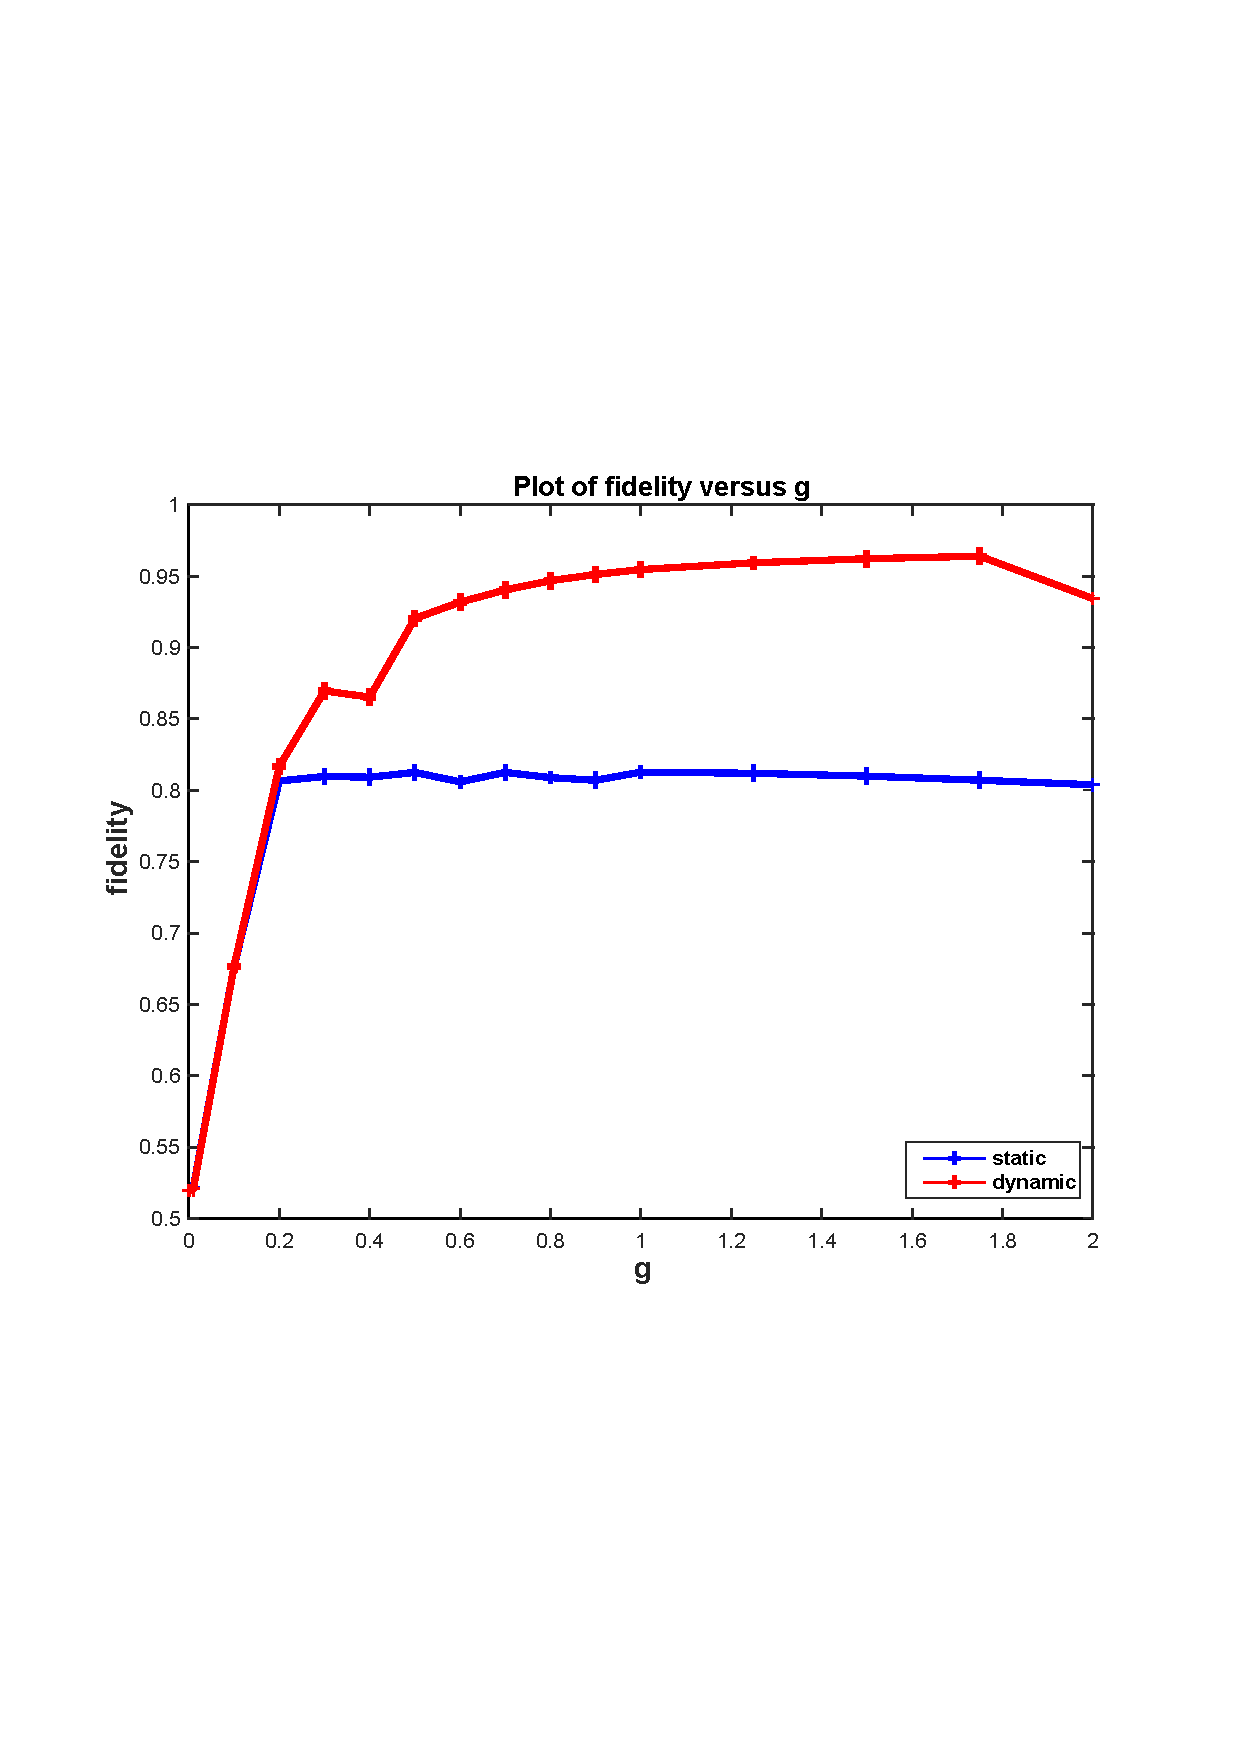
\includegraphics[width=1.1\textwidth]{F_both_in_one}
\caption{Plot of fidelity versus g(coupling strength) for both dynamic as well as static}
\label{F_both_in_one}
\end{figure}
\end{center}
%\lipsum[4-7]


\begin{center}
\begin{figure}%[!h]
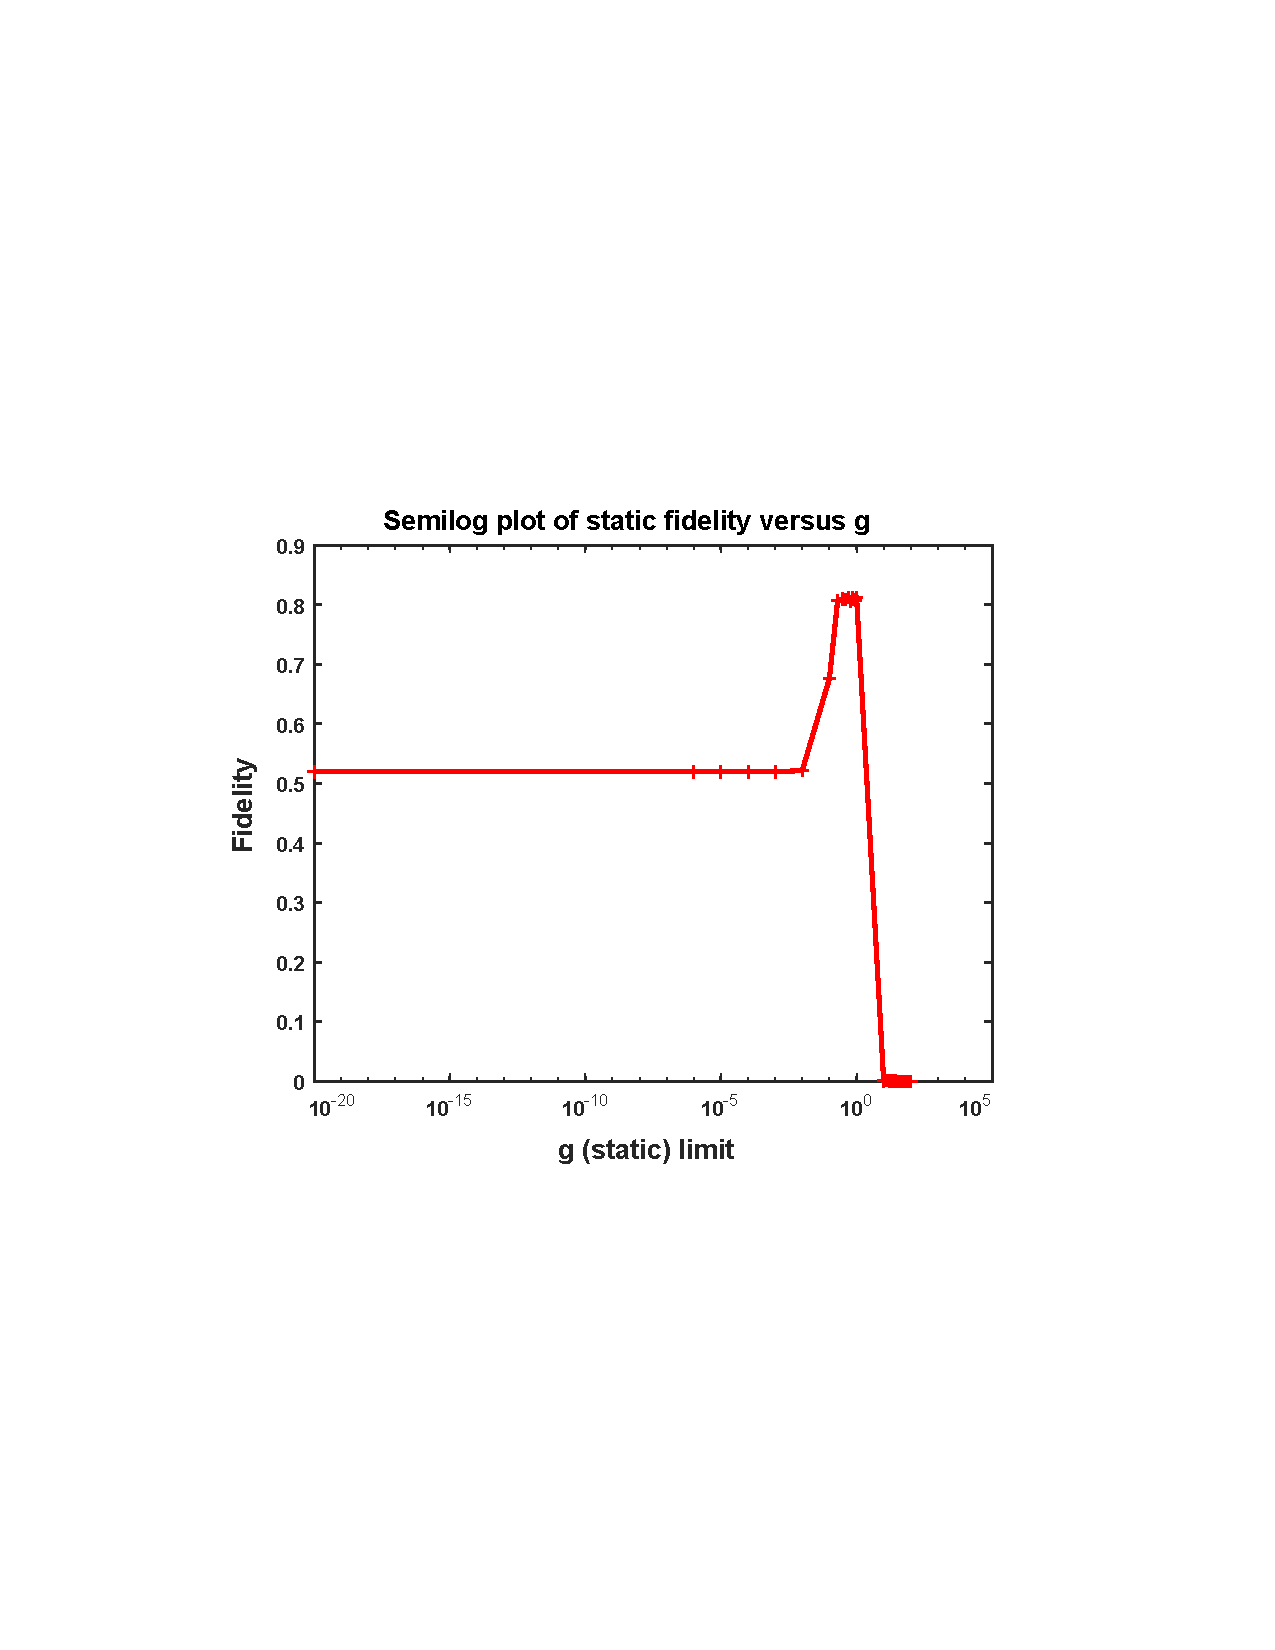
\includegraphics[width=1.1\textwidth]{A_fidelity_static_g__semilog_large_range}
\caption{Semi logarithmic plot of static fidelity versus g(coupling strength). This is plot of the target state fidelity obtained versus the coupling strength. g. For each of the above data points the coupling strength is held at a fixed value for the entire length of the time the system is allowed to evolve. At a time, $t = t_{max}$. we measure the overlap of the target state with the final state in terms of the fidelity metric.}
\label{A_fidelity_static_g__semilog_large_range}
\end{figure}
\end{center}
%\lipsum[4-7]


\begin{center}
\begin{figure}%[!h]
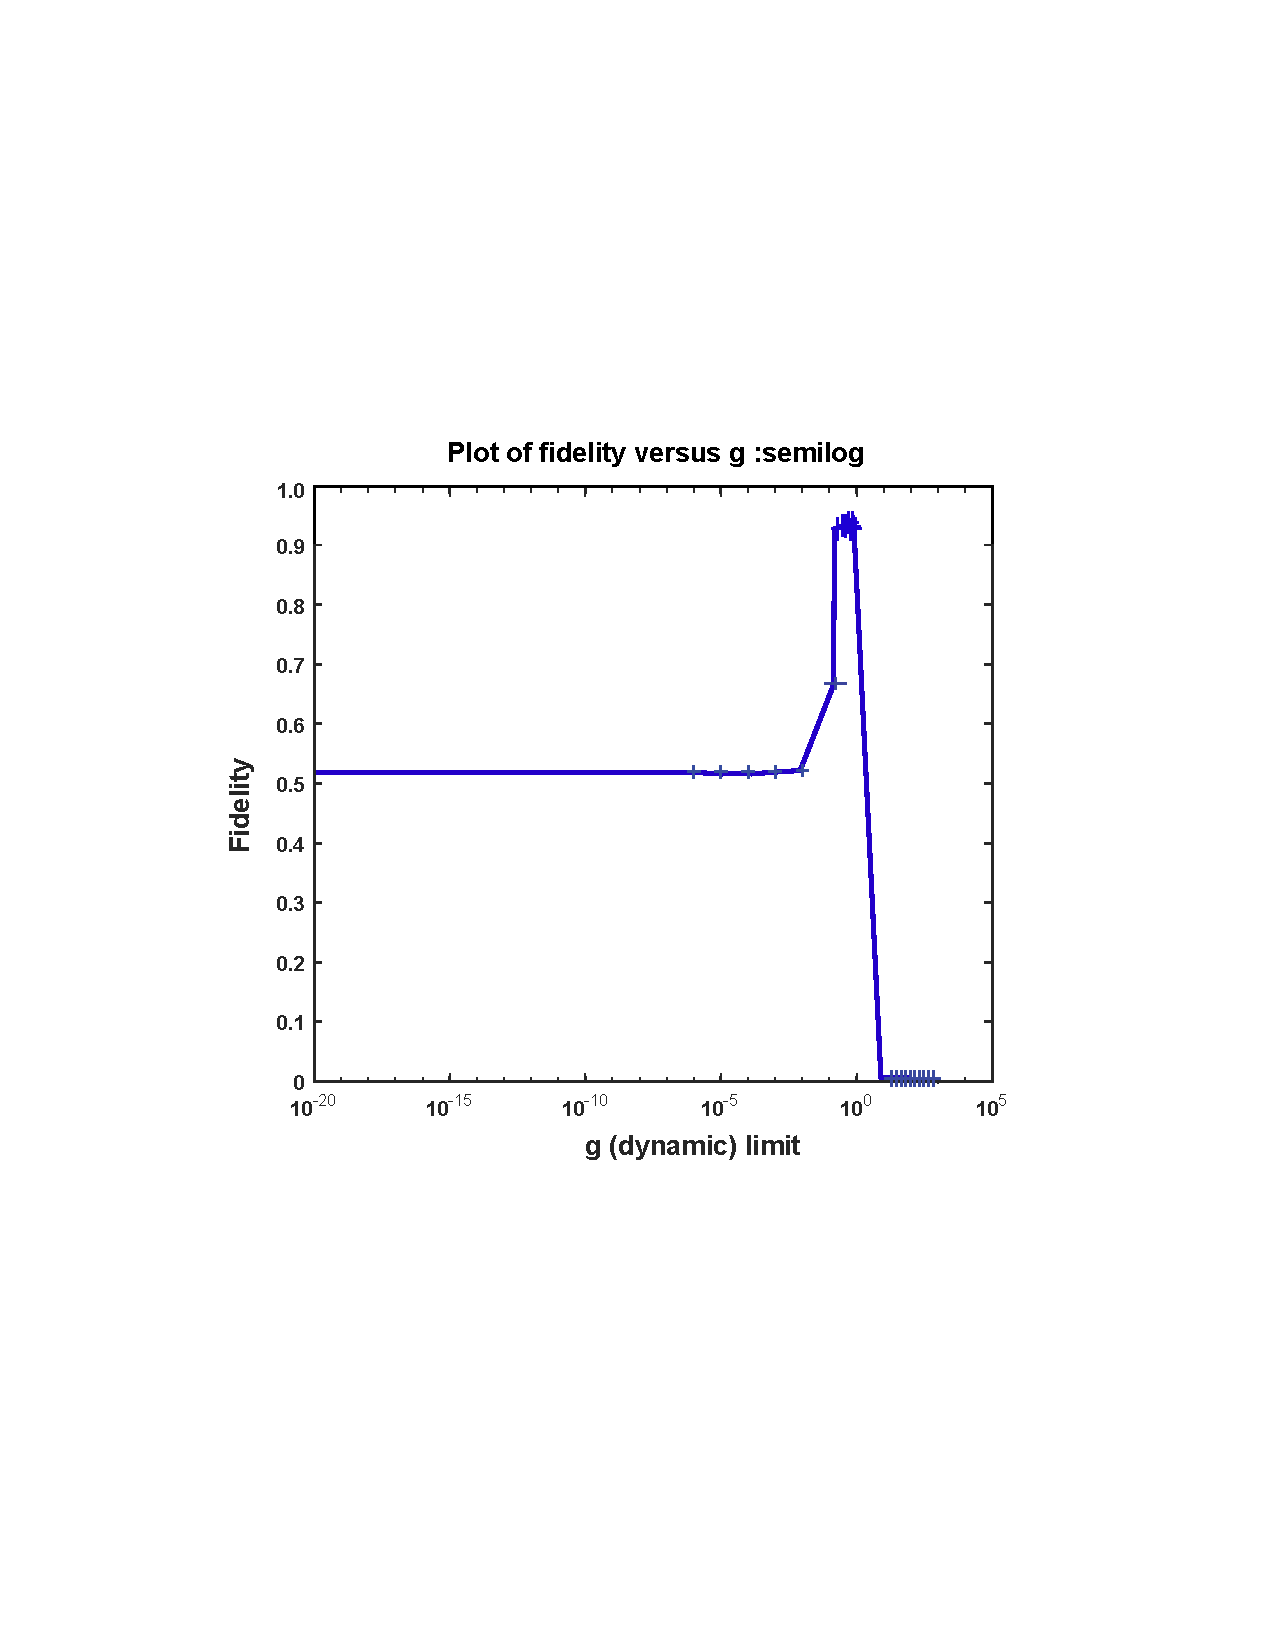
\includegraphics[width=1.1\textwidth]{H-fk_fidelity_static_g__semilog_large_range_-_Final}
\caption{Semi logarithmic plot of dynamic fidelity versus g(coupling strength). This is a plot of the target state fidelity obtained versus the maximum value of the coupling constant $g_{max}$ during the particular run. The coupling strength is varied with time such that the maximum value  in a particular run is less than or equal to $g_{max}$. This is true for all the data points. At time $t=t_{max}$ one measures the over lap of the target state to the state of the system at $t=t_{max}$ in terms of fidelity metric.     }
\label{H-fk_fidelity_static_g__semilog_large_range_-_Final}
\end{figure}
\end{center}
%\lipsum[4-7]

\begin{center}
\begin{figure}%[!h]
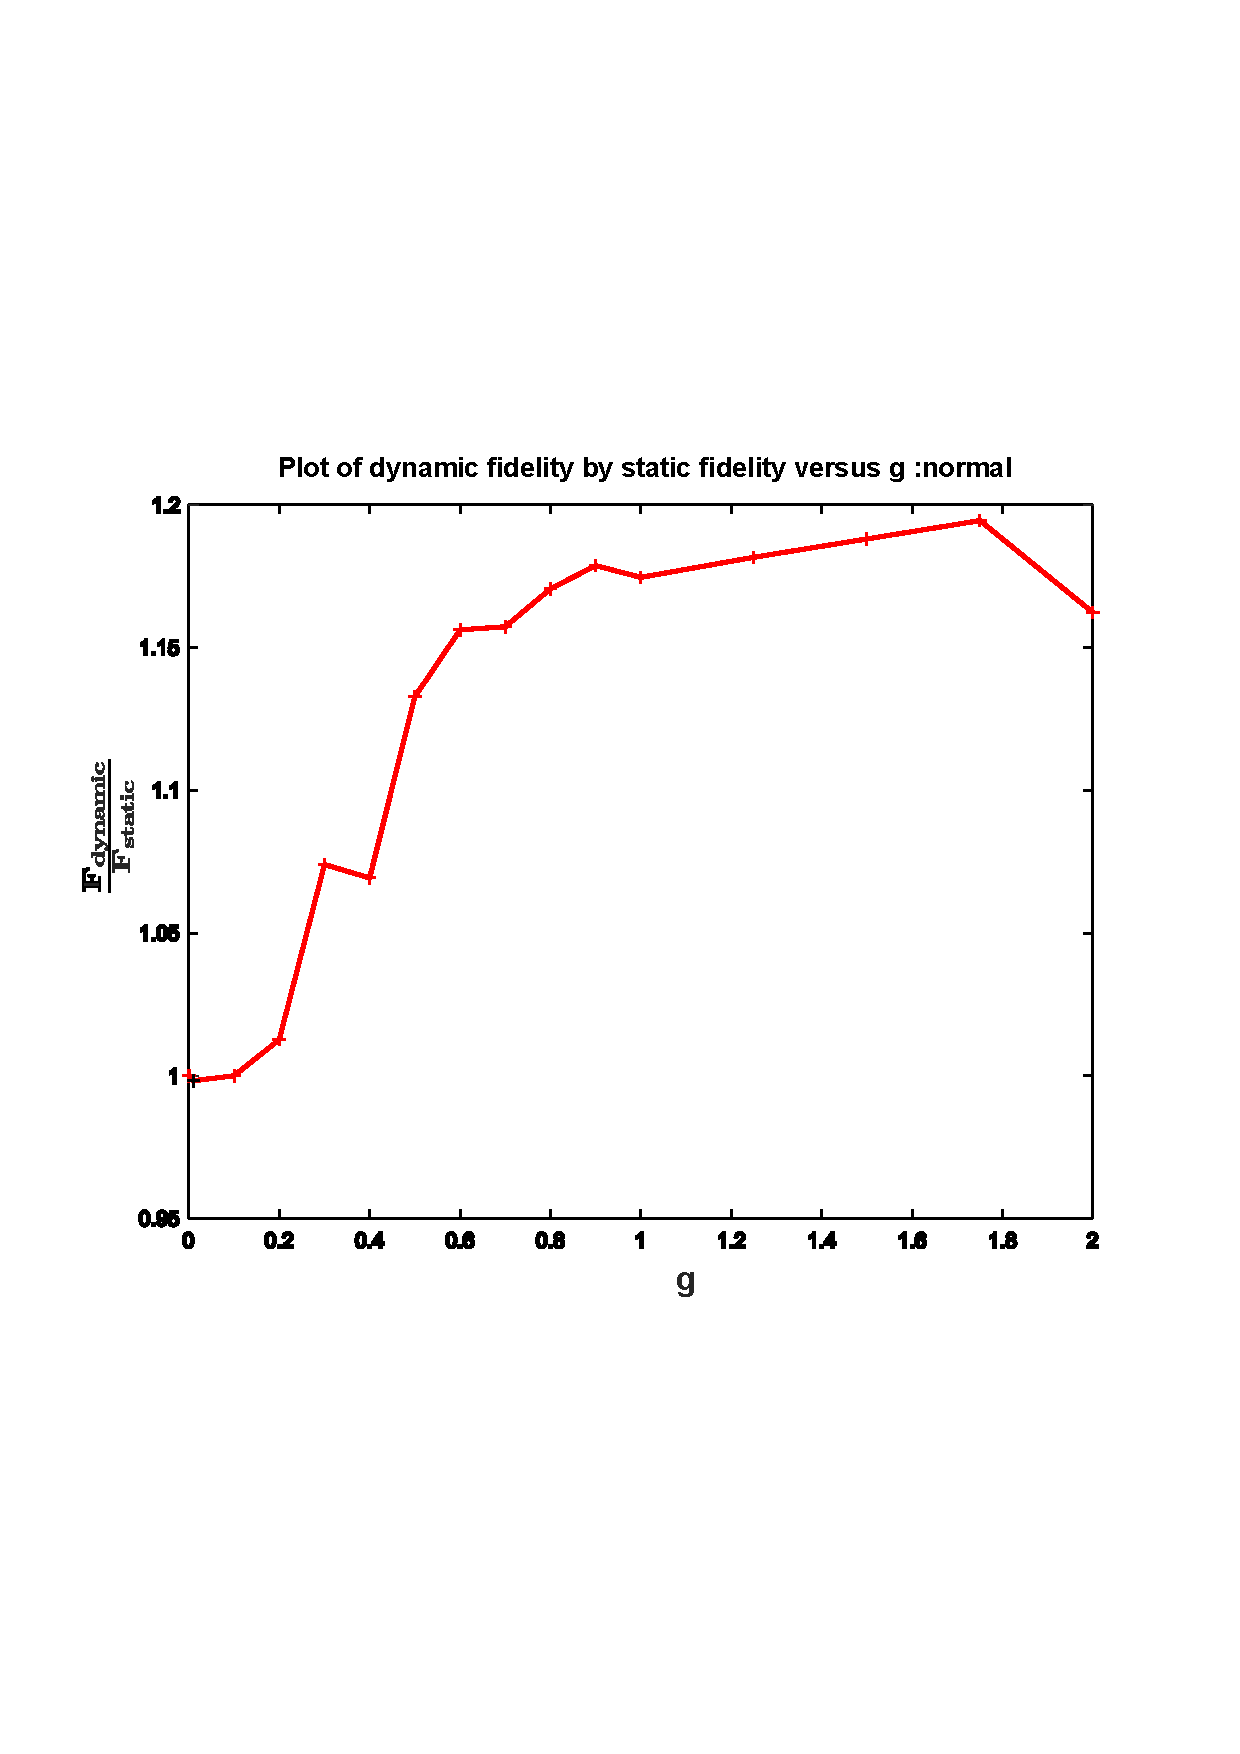
\includegraphics[width=1.1\textwidth]{E_dynamic_static_versus_g__normal}
\caption{Plot of ratio of dynamic fidelity by static fidelity versus g(coupling strength)}
\label{E_dynamic_static_versus_g__normal}
\end{figure}
\end{center}
%\lipsum[4-7]










\begin{comment}
\begin{center}
\begin{figure}%[!h]
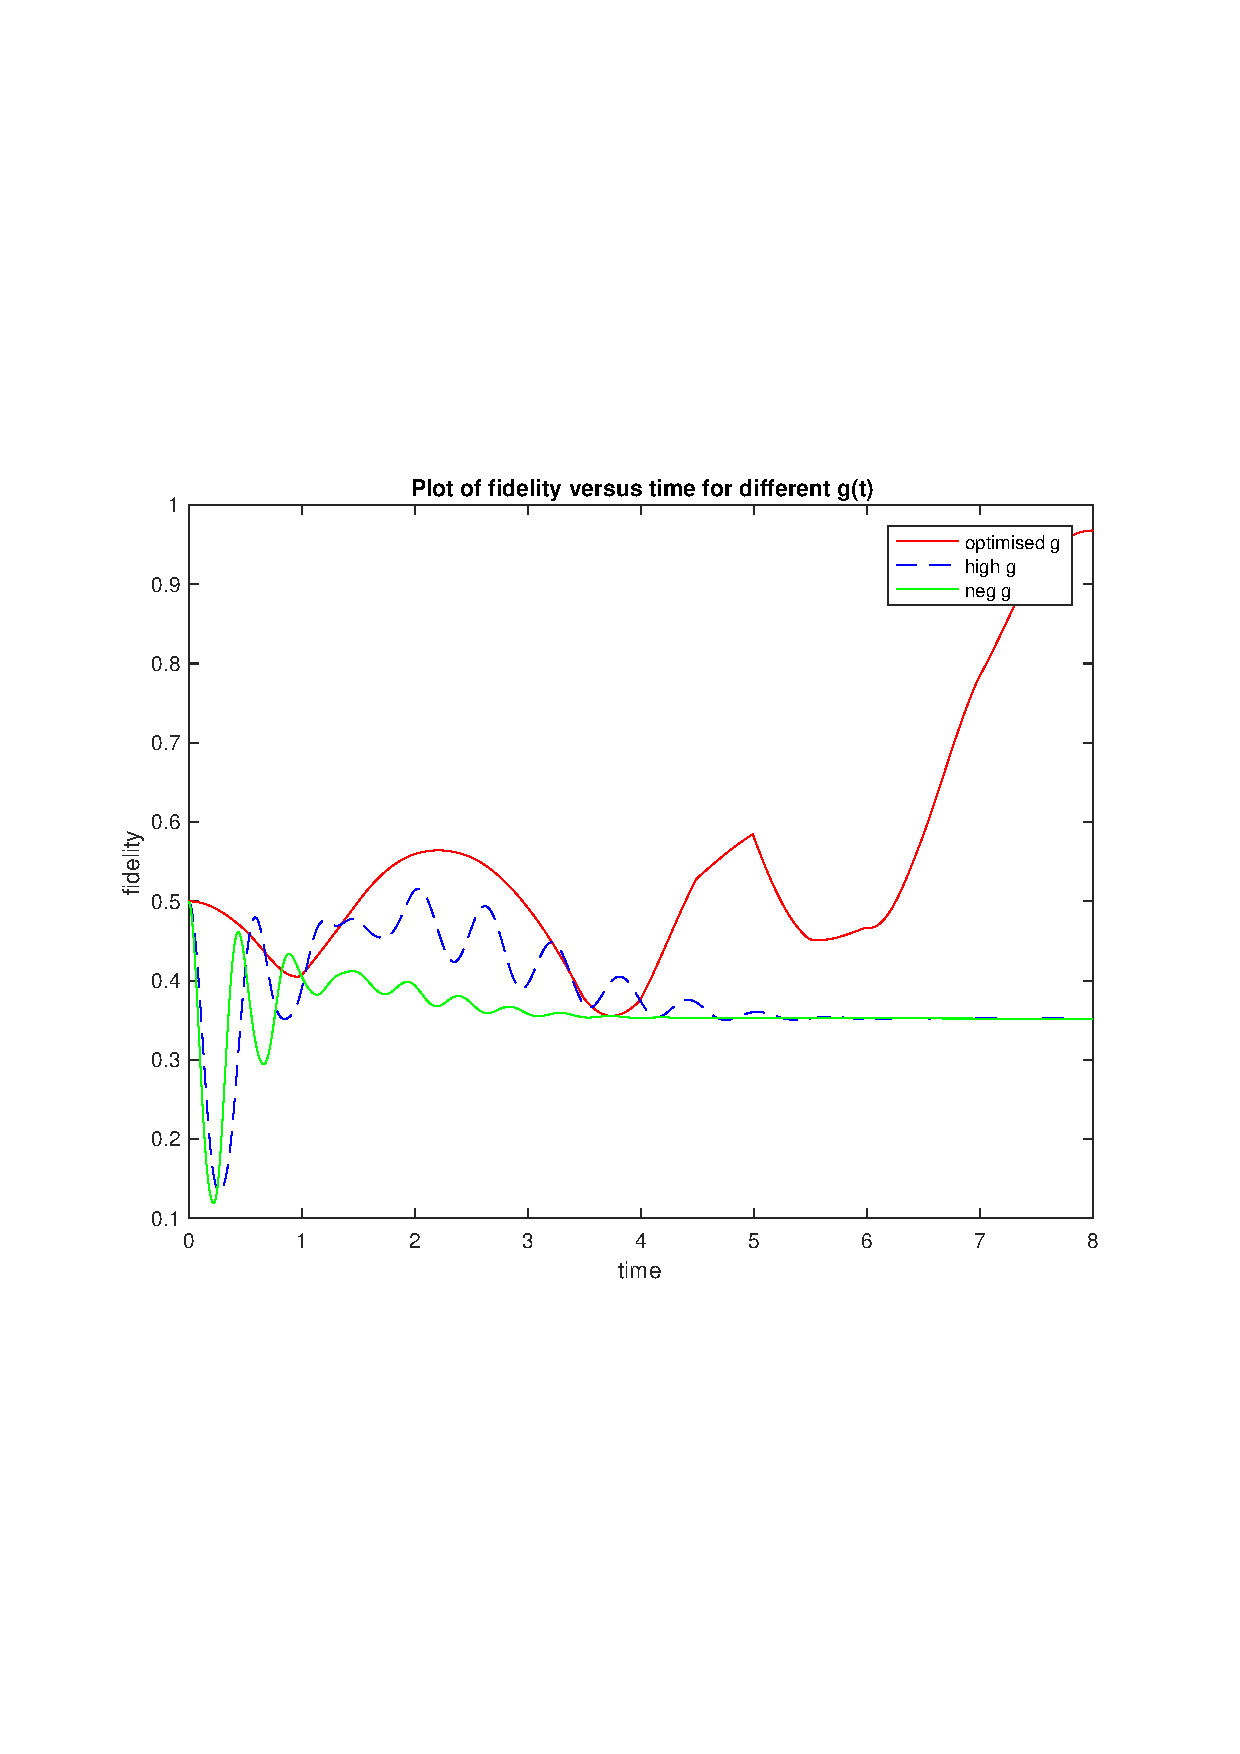
\includegraphics[width=1.0\textwidth]{gvary7}
\caption{Plot of fidelity versus time for different   g (t) }
\label{fig:gvary7}
\end{figure}
\end{center}
%\lipsum[4-7]
\end{comment}













\begin{comment}

\newpage
\begin{center}
\begin{figure}%[!h]
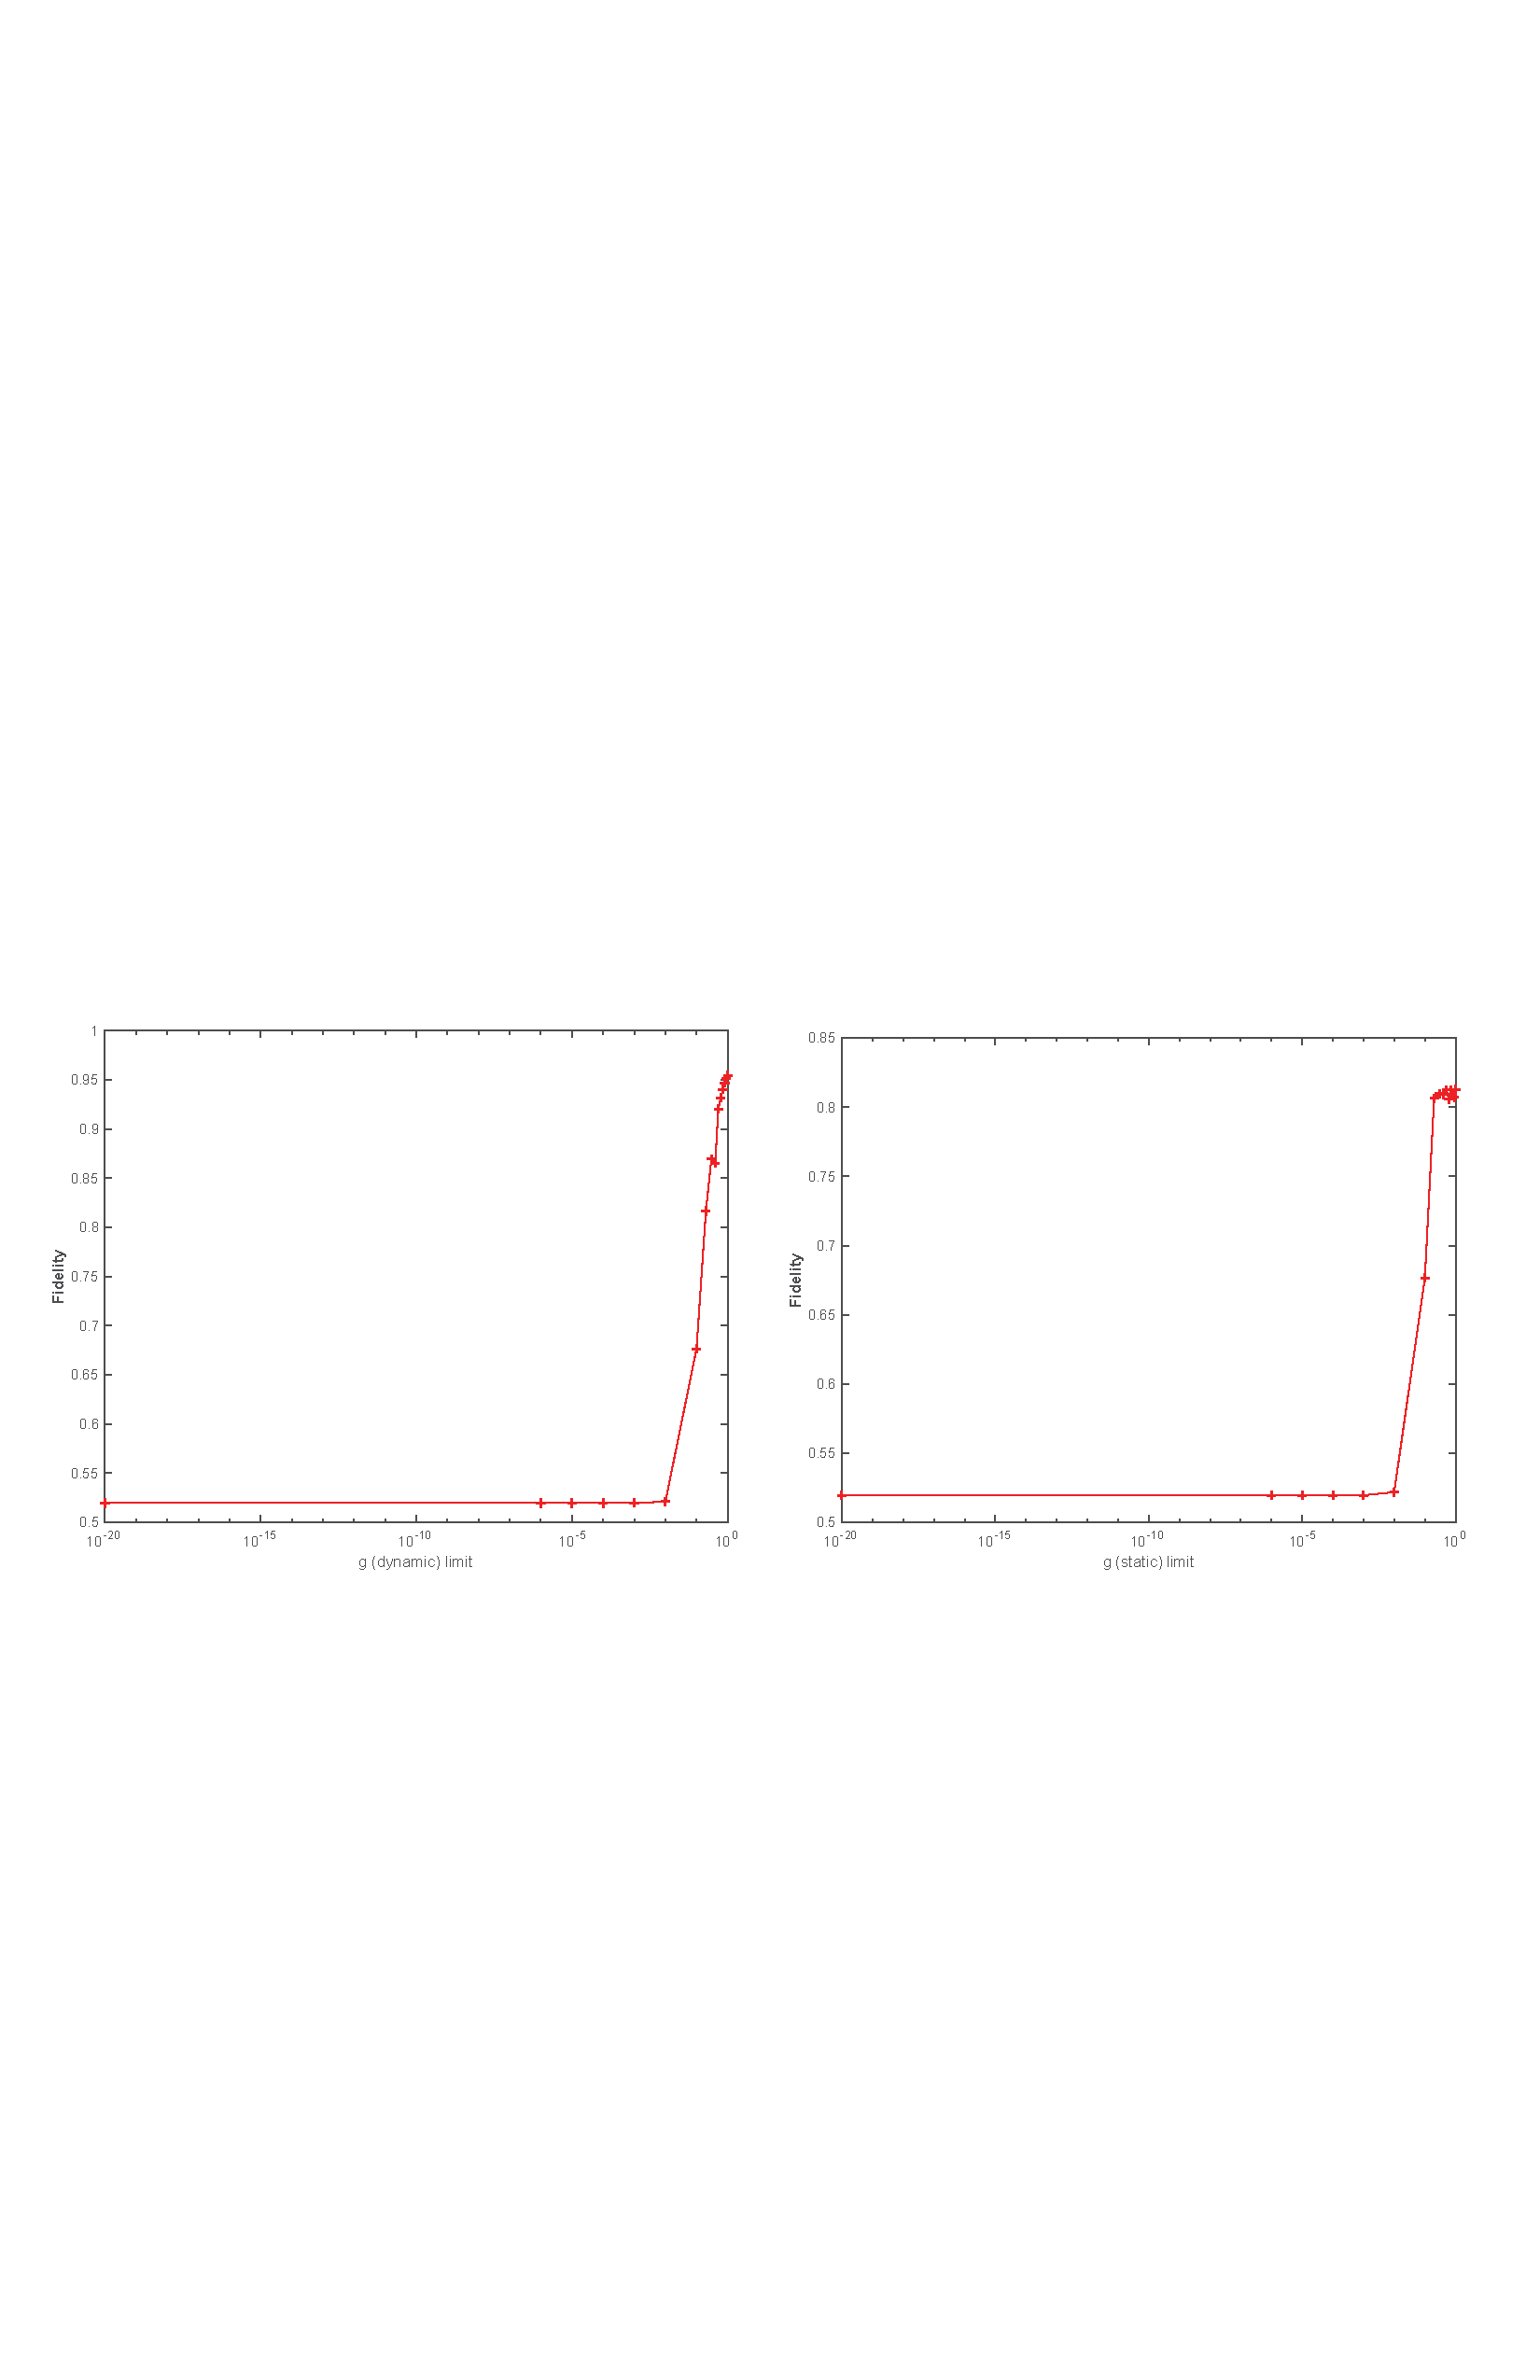
\includegraphics[width=1.1\textwidth]{Integrated_2_graph}
\caption{Semi logarithmic plot of fidelity versus g(coupling strength) for both dynamic as well static. Please note the different scales in Y axis.}
\label{fig:Integrated_2_graph}
\end{figure}
\end{center}
%\lipsum[4-7]





\begin{center}
\begin{figure}%[!h]
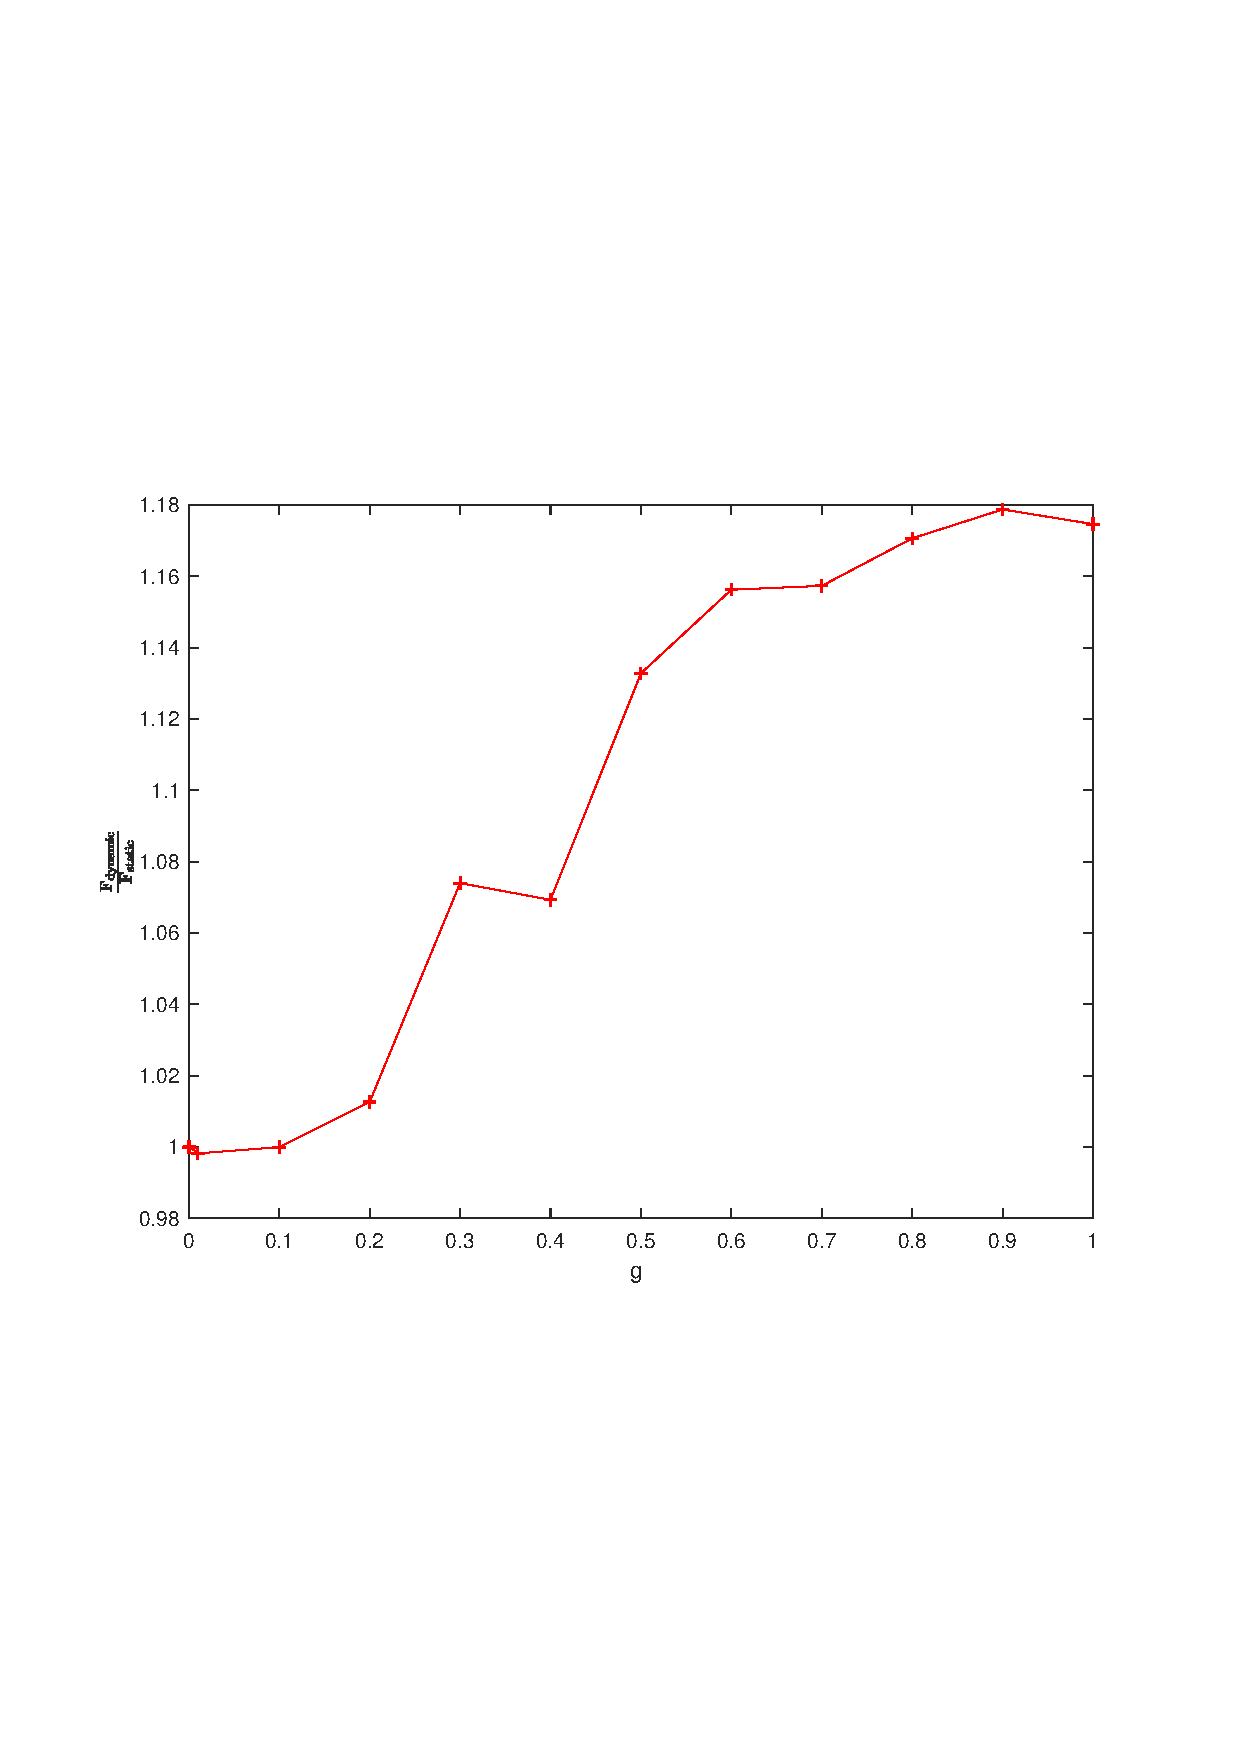
\includegraphics[width=1.0\textwidth]{25-19feb-advantage_normal1}
\caption{Plot of dynamic by static versus g(coupling strength) : normal  }
\label{fig:25-19feb-advantage_normal1}
\end{figure}
\end{center}
%\lipsum[4-7]

\begin{center}
\begin{figure}%[!h]
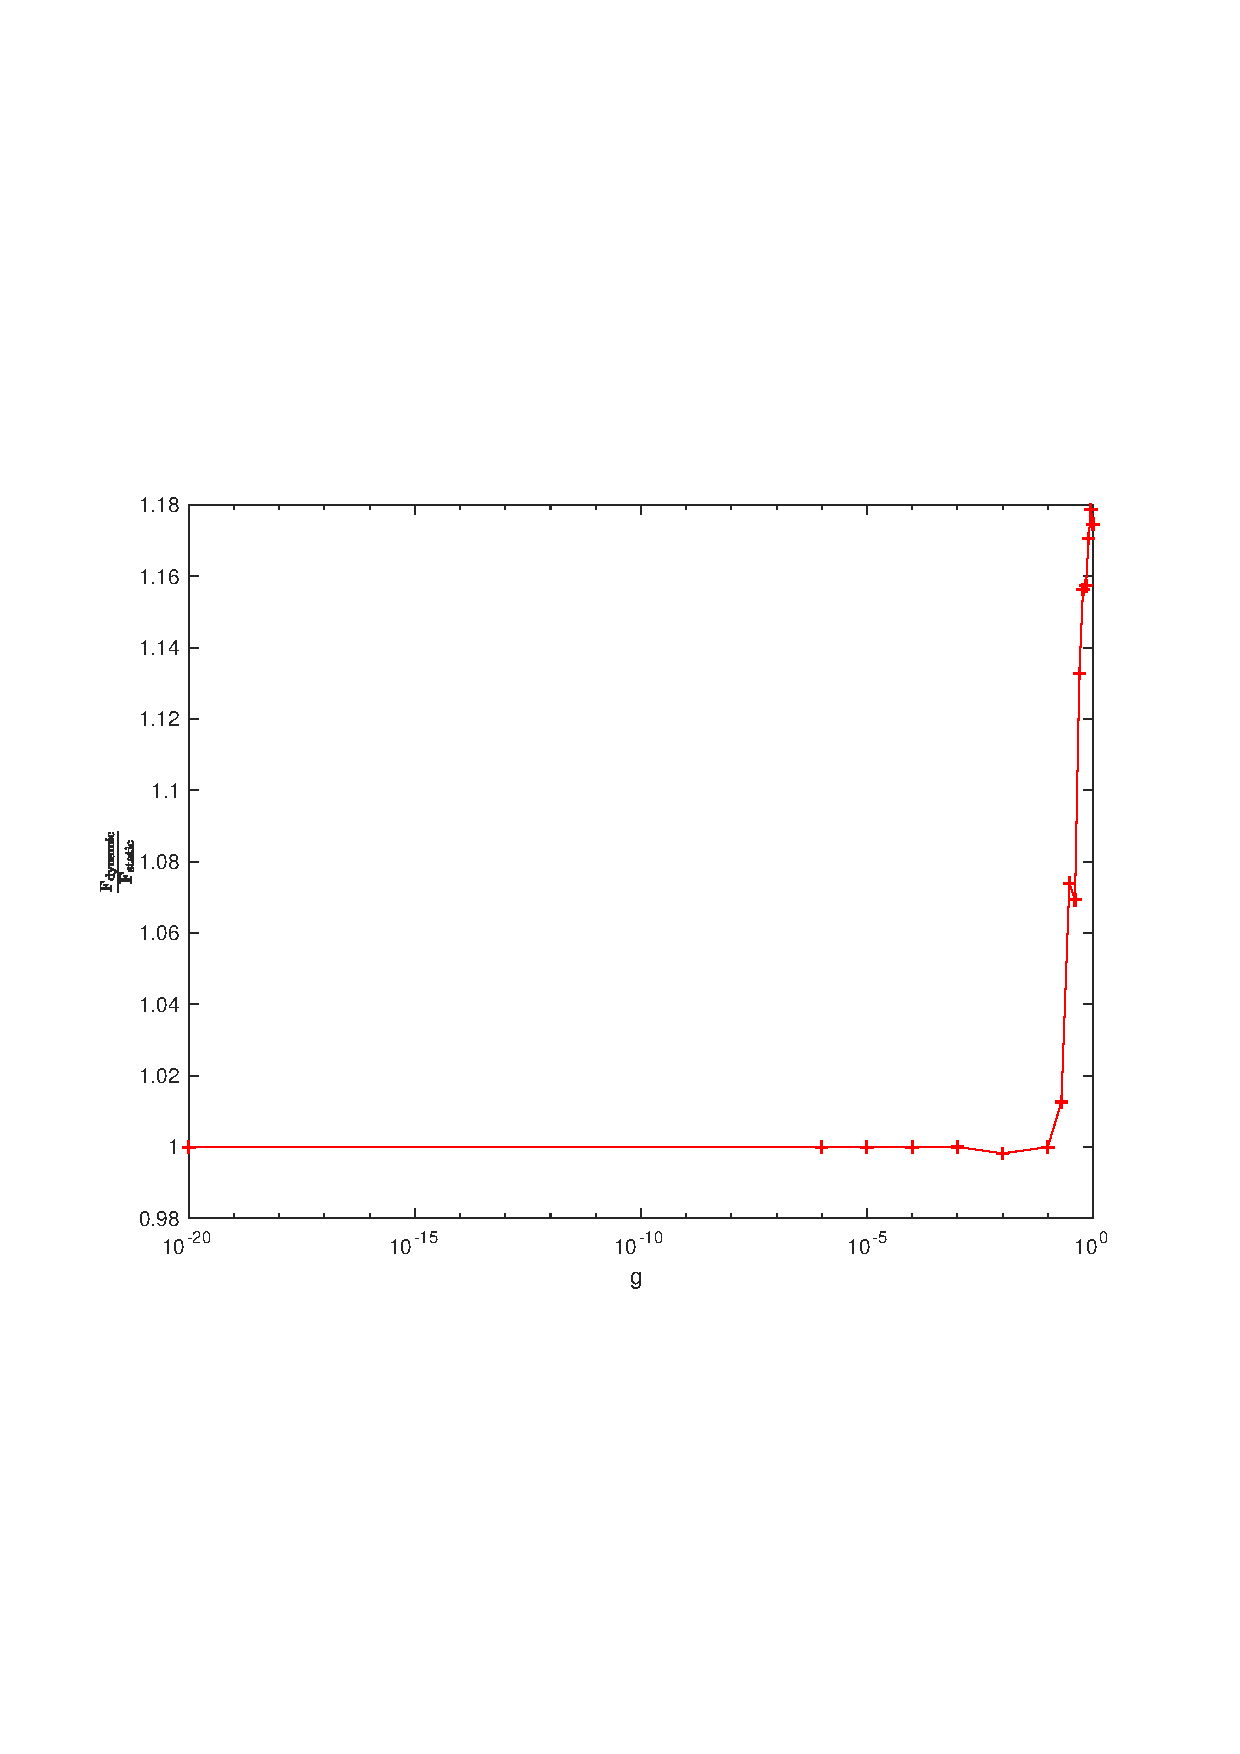
\includegraphics[width=1.0\textwidth]{26-19feb-advantage_semilog}
\caption{Plot of dynamic by static versus g(coupling strength) : semilog }
\label{fig:26-19feb-advantage_semilog}
\end{figure}
\end{center}
%\lipsum[4-7]

\end{comment}
















\begin{comment}



\begin{center}
\begin{figure}%[!h]
\includegraphics[width=1.0\textwidth]{29-19feb-fidelity_dynamic_g__normal}
\caption{Plot of fidelity versus g:normal}
\label{29-19feb-fidelity_dynamic_g__normal}
\end{figure}
\end{center}
%\lipsum[4-7]

\begin{center}
\begin{figure}%[!h]
\includegraphics[width=1.0\textwidth]{30-19feb-fidelity_dynamic_g__semilog}
\caption{Plot of fidelity versus g :semilog}
\label{30-19feb-fidelity_dynamic_g__semilog}
\end{figure}
\end{center}
%\lipsum[4-7]


\begin{center}
\begin{figure}%[!h]
\includegraphics[width=1.0\textwidth]{31-19feb-fidelity_static_g__normal}
\caption{Plot of fidelity versus g :normal   :normal}
\label{31-19feb-fidelity_static_g__normal}
\end{figure}
\end{center}
%\lipsum[4-7]


\begin{center}
\begin{figure}%[!h]
\includegraphics[width=1.0\textwidth]{32-19feb-fidelity_static_g__semilog}
\caption{Plot of fidelity versus g :semilog }
\label{32-19feb-fidelity_static_g__semilog}
\end{figure}
\end{center}
%\lipsum[4-7]


\begin{center}
\begin{figure}%[!h]
\includegraphics[width=1.0\textwidth]{7-fidelity_dynamic_g__normal}
\caption{Plot of fidelity versus g :normal}
\label{7-fidelity_dynamic_g__normal}
\end{figure}
\end{center}
%\lipsum[4-7]


\begin{center}
\begin{figure}%[!h]
\includegraphics[width=1.0\textwidth]{9-fidelity_static_g__normal}
\caption{Plot of fidelity static g :normal  :}
\label{9-fidelity_static_g__normal}
\end{figure}
\end{center}
%\lipsum[4-7]

\end{comment}



\begin{comment}



\begin{center}
\begin{figure}%[!h]
\includegraphics[width=1.0\textwidth]{27-19feb-dynamic_static_versus_g__normal}
\caption{Plot of dynamic by static versus $g$  :normal}
\label{27-19feb-dynamic_static_versus_g__normal}
\end{figure}
\end{center}
%\lipsum[4-7]


\begin{center}
\begin{figure}%[!h]
\includegraphics[width=1.0\textwidth]{28-19feb-dynamic_static_versus_g__semilog}
\caption{Plot of dynamic by static versus $g$ :semilog  }
\label{28-19feb-dynamic_static_versus_g__semilog}
\end{figure}
\end{center}
%\lipsum[4-7]


\begin{center}
\begin{figure}%[!h]
\includegraphics[width=1.0\textwidth]{33-19feb-fidelity_versus_g__normal}
\caption{Plot of fidelity versus g :normal$g$ }
\label{33-19feb-fidelity_versus_g__normal}
\end{figure}
\end{center}
%\lipsum[4-7]




\begin{center}
\begin{figure}%[!h]
\includegraphics[width=1.0\textwidth]{34-19feb-fidelity_versus_g__semilog}
\caption{Plot of fidelity versus $g$:semilog }
\label{34-19feb-fidelity_versus_g__semilogl}
\end{figure}
\end{center}
%\lipsum[4-7]












\begin{figure}
\centering
\includegraphics[width=0.8\textwidth]{1-16feb11.pdf}
\caption{1-16feb11}
\label{fig:1-16feb11}
\end{figure}

\begin{figure}
\centering
\includegraphics[width=0.8\textwidth]{1-16feb11-001.pdf}
\caption{1-16feb11-001}
\label{fig:1-16feb11-001}
\end{figure}


\begin{figure}
\centering
\includegraphics[width=0.8\textwidth]{11-runwith100000.pdf}
\caption{11-runwith100000}
\label{fig:11-runwith100000}
\end{figure}

\begin{figure}
\centering
\includegraphics[width=1.0\textwidth]{5-16feb12.pdf}
\caption{5-16feb12}
\label{fig:5-16feb12}
\end{figure}


\begin{figure}
\centering
\includegraphics[width=1.0\textwidth]{8-16feb6.pdf}
\caption{8-16feb6}
\label{fig:8-16feb6}
\end{figure}

\begin{figure}
\centering
\includegraphics[width=1.0\textwidth]{2-16feb15.pdf}
\caption{2-16feb15}
\label{fig:2-16feb15}
\end{figure}

\begin{figure}
\centering
\includegraphics[width=1.0\textwidth]{3-16feb16.pdf}
\caption{3-16feb16}
\label{fig:3-16feb16}
\end{figure}
\lipsum[1-3]
\end{comment}








\chapter{Current progress}
Recent developments in quantum dot based qubits have managed to convince us that good quality qubits are just around the corner. \cite{petta} have managed to synthesize Si double quantum dot based qubits which have strong coupling between the single electron in the dot to the photonic field of a microwave cavity. This allows for entanglement and coupling over large distances. This enables us to envision devices which are quantum coupled or entangled with each other even if far away from each other. 
\par
Anyway coming back to the point, their set up is a double quantum dot qubit placed in a microwave cavity. This is quite similar to our setup in which we have two qubits place in a cavity.\\ 
\begin{figure}
\centering
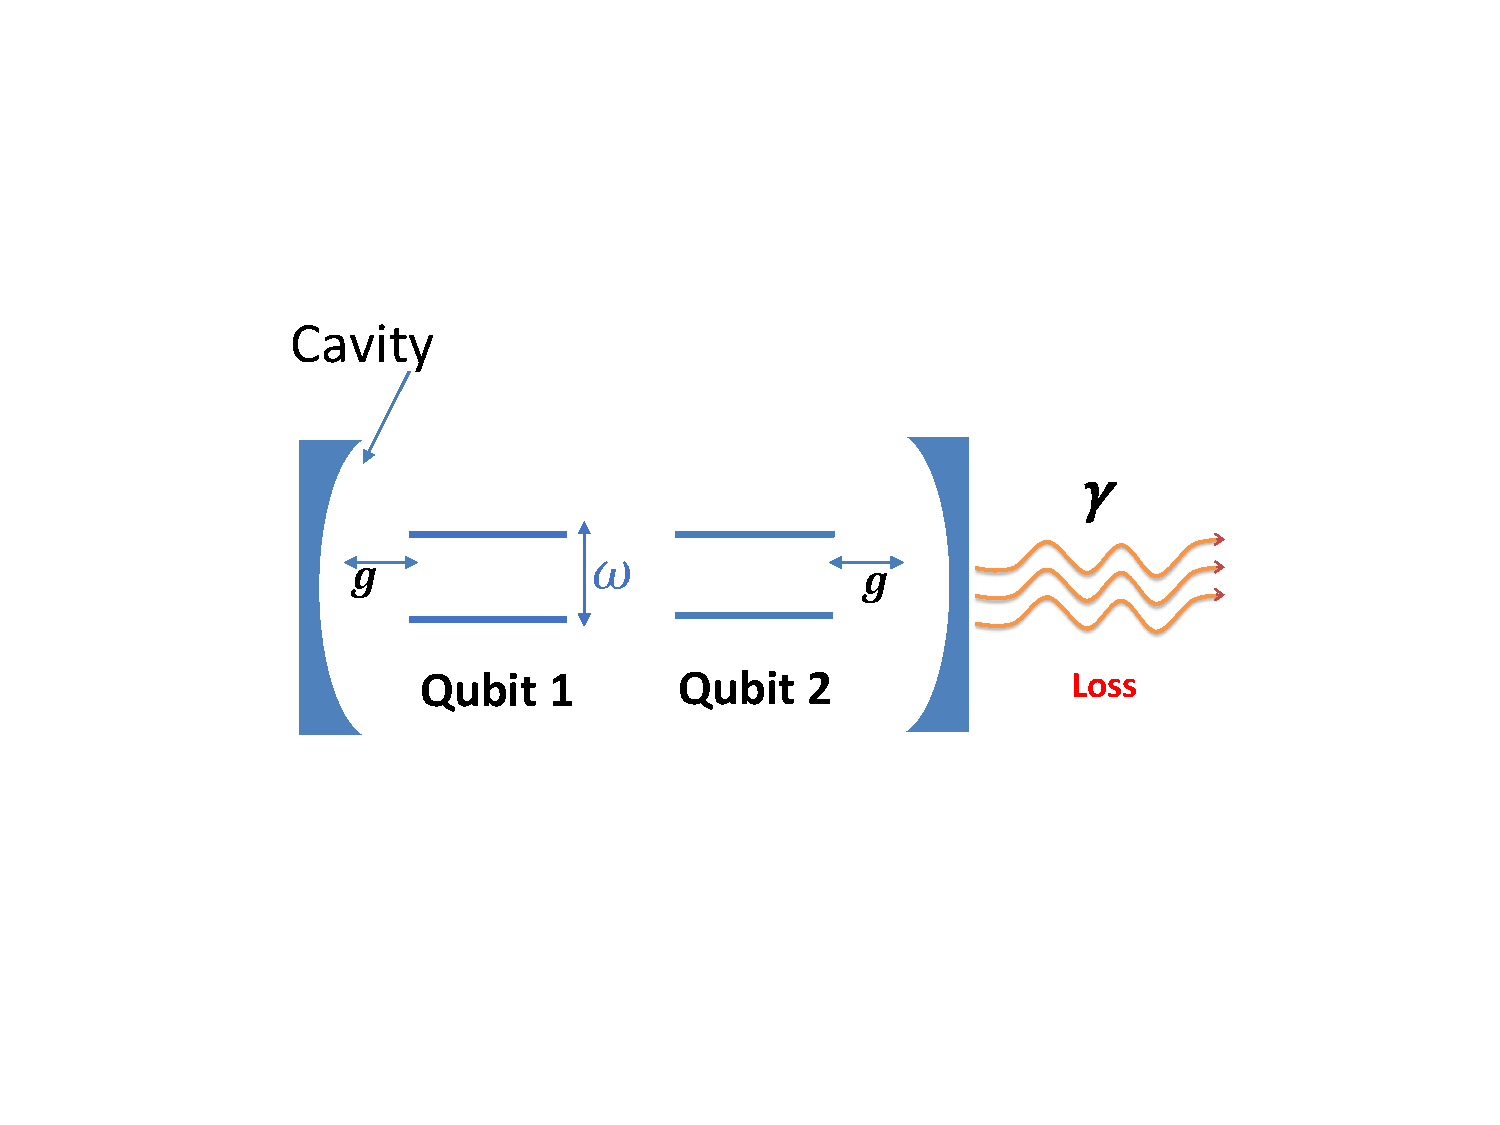
\includegraphics[width=0.8\textwidth]{Figr1a} 
\end{figure}
\par
The range of $\omega_{c}$ is about the range of $\omega_{q}$.  As we saw last time it is better to vary the field $g(t)$. Only if it is specific range and not otherwise looking for answers we hit upon \cite{hot_gates}. By performing certain algebraic manipulations they manage to decouple the qubits from the cavity at specific intervals of time. The only way the qubits interact is via the cavity. If one moves the cavity there wont be any path by which they could decohere.This brings about long coherence times, and allows on to operate at "elevated temperatures" 1K to 4K. These temperatures are far higher than what one usually encounters in this field eg.mK. It also would allow us to make classical connections to quantum hardware.Here their system is exactly the same as ours but they require that the qubit level spacing $\omega_{q}$ is less than of $\omega_{c}$. This puts it out of the range of \cite{petta}.
\par
Basically we need a way in which one could efficiently develop control field temporal variation to implement a specific gate.  It must be like an algorithm where on performing a series of steps either repeatedly or otherwise one ends up with a control field that performs the unitary we want. This it must be able to do to a tolerable (practical) level of error. Few of the algorithms that do this are:
\begin{itemize}
    \item Krotov as in \cite{tannor1992control}
    \item \cite{zhu1998rapid}
    \item GRAPE  \cite{khaneja2005optimal}
    \item CRAB (Chopped RAndom Basis) \cite{doria}, \cite{caneva2011chopped}
    \item DCRAB (Dressed Chopped RAndom Basis) \cite{rach2015dressing}
    \item GOAT (Gradient Optimization of Analytic conTrols) \cite{machnes2015gradient}
\end{itemize}
\par
Krotov \citep{tannor1992control} and \citep{zhu1998rapid} were combined together in a single algorithm by \citep{maday2003new}.   GRAPE \citep{khaneja2005optimal} is Gradient Ascent by Pulse Engineering. It explicitly makes use of derivatives. When unable to do so it calculates a suitable thing which emulates them. Primarily they are gradient descent algorithms. They always get a solution but sometimes require appalling amount of computational resources. CRAB and its improvements DCRAB \citep{rach2015dressing} are basically non gradient methods which make use of analytic functions. These methods have may fail to reach the optimal solution but do so quickly on being successful.
\par
GOAT  \citep{machnes2015gradient} combines the best features of all before it to achieve high accuracy without compromising on speed. It is some what more complicated though.
\par
To keep things simple lets start with Krotov by \citep{tannor1992control} algorithm in the form given by  \citep{maday2003new}. To gain deeper understanding, first we must generalize our system. So instead of   

   





\section{Introduction}
 Say, we want to apply a target unitary $T_{s} $ on our quantum system. Let the Hamiltonian of our system be $\mathcal{H} $. The Lindbladian operators associated with it be $\{ L_{m} \}$. The Hamiltonian of the system is given by 
\begin{align}\label{Hamiltonian form}
    H &= H_{0} + g(t) H_{I} 
\end{align}

where,
\begin{enumerate}
    \item[$H_{0} :$] bare Hamiltonian
    \item[$ g(t) :$] control field as a function of time.
    \item[$ H _{ I} :$] control Hamiltonian (interaction Hamiltonian)
\end{enumerate}

The system is assumed to be governed by Lindblad equation.
\begin{align}
    \dot{\rho} = - i\comm{H}{\rho} + \mathcal{L}(\rho)
\end{align}

where,
\[
 \mathcal{L}(\rho) = \gamma\sum_{m} L_{m}\thinspace \rho L_{m}^{\dagger} - 0.5 \anticommutator{L_{m}^{\dagger}L_{m}}{ \rho}
\]

The application of a target unitary $T_{s} $ on the system can be translated in mathematical terms (in open quantum systems formalism) as follows :
\[
 \rho \rightarrow T_{s}\thinspace  \rho T_{s} ^{\dagger}
\]
%https://www.overleaf.com/1524532912qjmbpfcwcpbv
So, the question at hand is what must be the form of $ g (t)$
 such that for any $\rho $ if we let the system evolve (under the influence of the  control field  $g (t) $ ) we get the final state $T_{s} \rho  T_{s} ^{\dagger}$.

\section{Taking advice from other sources}
%Some advice from \cite{2018EPJST.227..203S}
\cite{2018EPJST.227..203S} have  discussed a similar problem with one major difference. Instead of implementing a specific unitary gate they have a fixed initial state which they wish to evolve to a fixed target state.  They wish to find know how would $ g(t)$ have to vary for the quantum system to evolve as close as possible to the target state. They discuss how this has already been done in many ways for closed quantum systems. The one which they focus upon is given in \cite{2012JChPh.136j4103R}.


Let us have quick review of it. Assuming we have a closed quantum system which we want to drive from a fixed state $ \ket{\psi _{0}}$ to a target state $ \ket{\tau} $. The Hamiltonian of the system is as in \eqref{Hamiltonian form}.
For this the write down a cost function $J$ as follows (details are in  \cite{2018EPJST.227..203S}) :
\begin{align}\label{cost_function}
    J[\ket{\psi}, \ket{\chi}, g(t)] &= \expval{Q}{\psi(T)} - 2Re\int_{0}^{T}dt \matrixelement{\chi(t)}{\dv{}{t} +  iH(t)}{\psi(t)}  - \alpha \int_{0}^{T}dt g^{2}(t)
\end{align}
where $ Q = \dyad{\tau}$. The first order variation $δJ$ is set to zero to obtain a set of equations, namely
\begin{align}\label{anal-krotov}
    i\ket{\dot{\psi}(t)} &=  H(t)\ket{\psi(t)},\text{with} \ket{\psi(0)} = \ket{\psi_{0}}\\
    i\ket{\dot{\chi}(t)} &= H(t)\ket{\chi(t)},\text{with} \ket{\chi(T)} = Q\ket{\psi(T)}\\
    g(t) &= \frac{-1}{\alpha}\text{Im}\matrixelement{\chi(t)}{\mu}{\psi(t)}
\end{align}


Following \cite{2012JChPh.136j4103R},   Eqns. \eqref{anal-krotov} could be solved self-consistently  as below,
\begin{align}\label{ansatz_krotov}
    i\ket{\dot{\psi}^{(k)}(t)} &=  H^{(k)}(t) \ket{\psi^{(k)}(t)},\text{with} \ket{\psi^{(k)}(0)} = \ket{\psi_{0}}\\
    i\ket{\dot{\chi}^{(k)}(t)} &= H^{(k)}(t) \ket{\chi^{(k)}(t)},\text{with} \ket{\chi^{(k)}(T)} = Q\ket{\psi^{(k)}(T)}\\
    g^{(k)}(t) &= (1 - \delta)\tilde{g}^{(k-1)}(t) -  \dfrac{\delta}{\alpha}\text{Im}\matrixelement{\chi^{(k-1)}(t)}{\mu}{\psi^{(k)}(t)}\\
    g^{(k)}(t) &= (1 - \eta)\tilde{g}^{(k)}(t) -  \dfrac{\delta}{\alpha}\text{Im}\matrixelement{\chi^{(k)}(t)}{\mu}{\psi^{(k)}(t)}
\end{align}

For open quantum systems \cite{2018EPJST.227..203S} suggest to move from the Hilbert space to Liouville space, which involves vectorizing the density matrix $\rho$ as $\ket{\psi}\rangle$. So the problem goes from 
 \begin{align}\label{Hilbert_liou:1}
     \rho_{0} &\rightarrow \rho_{f}\\
     \dot{\rho} &= - i\comm{H}{\rho} + \gamma\sum_{m} \left(L_{m} \rho L_{m}^{\dagger} - 0.5 \anticommutator{L_{m}^{\dagger}L_{m}}{ \rho}\right)\\
\text{to, }   
    \ket{\psi_{0}}\rangle &\rightarrow \ket{\tau}\rangle\\
    i\ket{\dot{\psi}(t)}\rangle &= A(t)\ket{\psi(t)}\rangle,  \text{ where}\\
    A(t) &= I\otimes H(t) - H^{*}(t)\otimes I + i\gamma\sum_{m} \left(
    L_{m}^{T}\otimes L_{m} - 0.5\left( I \otimes L_{m}^{\dagger} L_{m} + L_{m}^{T} L_{m}^{*} \otimes I\right)\right)
\end{align}
\section{Back to our problem}
Coming to our problem we have,
\begin{align}\label{Hilbert:2}
    \rho &\rightarrow T_{s}\thinspace\rho T_{s}^{\dagger}\\
    \dot{\rho} &= - i\comm{H}{\rho} + \gamma
    \sum_{m} \left(L_{m} \thinspace \rho L_{m}^{\dagger} - 0.5\anticommutator{L_{m}^{\dagger}L_{m}}{ \rho}\right)
\end{align}
Moving to Liouville space one can rewrite it as, 
 \begin{align}\label{Liouville:2}
     \ket{\psi}\rangle &\rightarrow T_{s}^{T} \otimes T_{s}\ket{\psi}\rangle\\
     i\ket{\dot{\psi}(t)}\rangle &= A(t)\ket{\psi(t)}\rangle
 \end{align}
where $A(t)$ is as given before in equation \eqref{Hilbert_liou:1}. From now on wards, let $T_{s}^{T} \otimes T_{s}$ be called as $T$.  But unlike \cite{2018EPJST.227..203S} instead of initial and final states we have the target unitary $T$. So, we cannot write the  same cost function and optimize it to get the desired control field. 
\section{Putting it all together}
Since,
\begin{align}
    i\ket{\dot{\psi}(t)}\rangle &= A(t)\ket{\psi(t)}\rangle\\
    \ket{\psi(t)}\rangle &= \mathcal{T}\left(e^{-i\int_{0}^{T} dt A(t)} \right)\ket{\psi(0)}
\end{align}
where $\mathcal{T}$ is the time ordering operator.
Let $\mathcal{T}\left(e^{-i\int_{0}^{T} dt A(t)} \right)$ be denoted by $\mathcal{L}$. One can approximate it as follows:
\begin{align}
    \mathcal{L}&=\mathcal{T}\left(e^{-i\int_{0}^{T}dt A(t)}\right)\\
    \mathcal{L}&= \prod_{k = N}^{1} \mathcal{L}_{k}\\
\end{align}
% $\mathcal{L}&=e^{-i\sum_{0}^{T}\delta t A(t)} = \prod_{k = N}^{1}$
where $\mathcal{L}_{k} = e^{-iA(t_{k})\delta t}$.
Let us define a few other terms.
\begin{align}\label{some_def}
    \mathcal{L}^{d}_{k} &= \mathcal{L}_{N}\mathcal{L}_{N-1}\ldots X_{k} \mathcal{L}_{k}\ldots \mathcal{L}_{2}\mathcal{L}_{1}\\
    X_{k} &= I\otimes H_{I} - H_{I}^{*}\otimes I 
\end{align}
%\phi &=  
%    J[g] &= -\phi^{*} \phi\\
Now we shall define $F[g] = - Tr((T - \mathcal{L})^{\dagger}(T - \mathcal{L}))$ to be our fidelity measure as in \cite{khaneja2005optimal}. Next we need to devise an update step for the control field which would improve the fidelity. Following \cite{khaneja2005optimal} we have 
\begin{align}\label{update_step}
    g(t_{k+1})&= g(t_{k}) + \epsilon\pdv{F}{g(t_{k})} \text{, or}\\
    g_{k+1} &=    g_{k}   + \epsilon\pdv{F}{g_{k}}
\end{align}
$\epsilon$ is  constant which would depend on the speed at which one would want to converge,etc.
\begin{align}
    \pdv{F}{g_{k}}&= -Tr((T - \pdv{\mathcal{L}}{g_{k}})^{\dagger}(T - \mathcal{L})) - Tr((T - \mathcal{L})^{\dagger}(T - \pdv{\mathcal{L}}{g_{k}})) \\
    \pdv{F}{g_{k}}&=  -Tr((T - \mathcal{L}^{d}_{k})^{\dagger}(T - \mathcal{L})) - Tr((T - \mathcal{L})^{\dagger}(T - \mathcal{L}^{d}_{k})))\\
    \mathcal{L}^{d}_{k}=\pdv{\mathcal{L}}{g_{k}} &= \pdv{(\mathcal{L}_{N}\mathcal{L}_{N-1}\ldots  \mathcal{L}_{k}\ldots \mathcal{L}_{2}\mathcal{L}_{1})}{g_{k}}\\
    \mathcal{L}^{d}_{k}=\pdv{\mathcal{L}}{g_{k}} &= \mathcal{L}_{N}\mathcal{L}_{N-1}\ldots \pdv{ \mathcal{L}_{k}}{g_{k}}\ldots \mathcal{L}_{2}\mathcal{L}_{1}\\
    \mathcal{L}^{d}_{k} &= \mathcal{L}_{N}\mathcal{L}_{N-1}\ldots X_{k} \mathcal{L}_{k}\ldots \mathcal{L}_{2}\mathcal{L}_{1}\\
    X_{k} &= I\otimes H_{I} - H_{I}^{*}\otimes I 
\end{align}
%$X_{k}$
\subsection{Steps to find optimal control field }
%$g_{opt}(t)$
\begin{enumerate}
    \item Start with a random $g_{rand}(t)$.
    \item Calculate fidelity $F$.
    \item Update $g(t) $ using  \Eqref{update_step}
    \item If fidelity $F$ calculated from new $g(t) $ differs from old one by more than $\mu$, then go to step 3.
    \item Terminate.
\end{enumerate}




%\chapter{Literature Survey}
Mike ike ,CRAB, DCRAB, GOAt etc biblio stuff already present in mylit.bib
The bibliographic entries are to be kept in a file named
\verb|<something>.bib|. In this sample report we call it as
\verb|mylit.bib|. This file must be included without the \verb|.bib|
extension in the main file as: \verb|\bibliography{mylit}|.   Open the
file \verb|mylit.bib| to see the format in which the entries are
written. This is written in the Bib\TeX format. Most of the
bibliographic web pages (Scopus, ISI Web) and software (EndNote, etc)
allow you to export bibliographic entries in the Bib\TeX format.

Citations are referred in the text using \verb|\citet| command which produces citations as though they are part of the text.  In order to say
somebody did this work as a part of a line use:
\verb|\citet{Batzri1973}| have done extensive work on \ldots.  This will produce
\citet{Batzri1973} have done extensive work on \ldots. Alternately citations can appear in parenthesis.  
The command~\verb|\citep{Batzri1973}| is used to automatically put the
citations in parenthesis.  As an example consider the extensive work
done in the area of book writing \citep{Sackmann1995a,Boal2012}.

Conferences \citep{rich-mart92} or collection of work
\citep{Sackmann1995a} also have special entries.

It is also possible to cite thesis like this:
\citet{jariwala00,luding94} or just unpublished work from
\citet{SunHI03}. Some times there are unclassified bibliographic
entries which can be put under ``misc'' \citep{Smith99}.
\citep{Whatisqubit} 
\citep{Tejas_APS1} \citep{wiki:resonator}

Tejas commonly used ones
\citep{nielsen2004quantum}
\citep{gerry2005introductory} \citep{caneva2011chopped} \citet{PaolaMIT2012}
\citep{2006quant.ph.12095L} \cite{jcreviewshoreknight}
@article{jcreviewshoreknight,
author = {Shore, Bruce and Knight, P},
year = {2018},
month = {09},
pages = {},
title = {Topical review The Jaynes-Cummings model}
}
URL citation format
\verb| @online{Whatisqubit,|\\
\verb|  author = {Margaret Rouse},|\\
\verb|  title = {DEFINITION qubit},|\\
\verb|  year = 2005,|\\
\verb|  url     = |\\
\verb|{\url{https://whatis.techtarget.com/definition/qubit}},|\\
\verb|  urldate = {2018-08-15}|\\
\verb|}|
can use verbatim environment for large blocks of text rather than  
\begin{verbatim}
\verb| |
 MIT OCW citation bibtex entry
 
@online{key,
  author = {Alan Oppenheim},
  year = {2011},
  month = {Spring},
  title = {Digital Signal Processing},
  subtitle = {RES.6-008},
  url = {https://ocw.mit.edu},
  organization = {Massachusetts Institute of Technology: MIT OpenCourseWare},
  addendum = {License: Creative Commons BY-NC-SA}
}
\end{verbatim}
Alan Oppenheim. RES.6-008 Digital Signal Processing. Spring 2011. Massachusetts Institute of Technology: MIT OpenCourseWare, https://ocw.mit.edu. License: Creative Commons BY-NC-SA.
%%% Local Variables: 
%%% mode: latex
%%% TeX-master: "../mainrep"
%%% End: 

%\chapter{Materials and Methods}

\section{Including Figures}

Figures are conveniently included using postscript  format.  If you are
generating a figure in a software, please check if the software
supports writing to a postscript or a PDF format. This format is loss
less vector format and with reproduce in any magnification without any
pixelation. Make sure to write it to an ``Encapsulated Post-script''or
.eps format.


\begin{figure}[tbp]
  \centering
    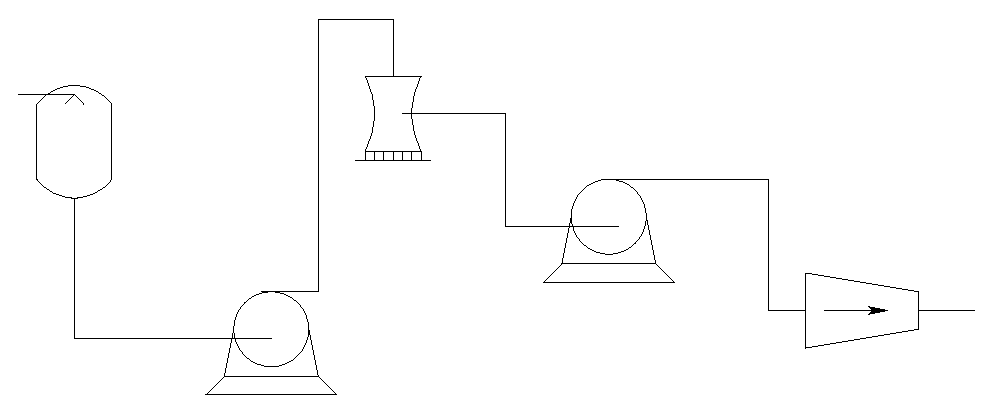
\includegraphics[width=0.7\textwidth]{profflow}
    \caption[Process flow sheet]{Process flow sheet of the
      experimental setup. The caption of the figure goes here. A
      shorter caption can be written in square brackets to identify it
      in the list of figures.}
    \label{fig:pfs} 
\end{figure}

Figures should be given a label and which can be used to refer to them
in the running text using \verb|\ref{}| command. Figure~\ref{fig:pfs}
describes the process flow sheet of the experimental set up used in
this report. The \Figref{fig:pfs} can also be refered by a short form notation
a pre-defined macro \verb"\Figref".



%%% Local Variables: 
%%% mode: latex
%%% TeX-master: "../mainrep"
%%% End: 

%\chapter{Results and Discussions}


\section{Including Tables}

Tables are to be used in a special environment so that they have a
Number, caption and appear in the list of tables.
Table~\ref{tab:samtab} is a sample table. In the case of tables, it is
a convention to write the caption above the table.  Note that in the
case of figures the caption appears below the figure.

\begin{table}[tbp]
  \centering
    \caption{Physical properties of the materials used.}
    \label{tab:samtab}
    \begin{tabular}{ll}
      \toprule 
      Property & Value \\
      \midrule
      Particle Density, $\rho_{\mathrm{p}}$ & 2500 kg/m$^{3}$ \\
      Viscosity, $\eta_{\mathrm{s}}$& 1 $\times 10^{-3}$ Pa-s \\
      \bottomrule \\
    \end{tabular}  
\end{table}

%%% Local Variables: 
%%% mode: latex
%%% TeX-master: "../mainrep"
%%% End: 

%\chapter{Conclusions}
Please write here the  broad conclusions and inferences drawn in the chapter on Results and Discussions. 
%****************************************************************
%                         Appendices                           
%****************************************************************
%% Additional, supporting material, such as codes, derivations, etc., can be placed in the appendix
%\appendix
%\chapter{Supporting Material}

%******************************************************************
%                         Bibliography or References          
%******************************************************************  
\bibliography{mylit}     

%*******************************************************************
%                         List of publications               
%******************************************************************
%%%%
\listofpublications


\noindent Put your publications from the thesis here. The packages \texttt{multibib} or \texttt{bibtopic} or \texttt{biblatex} or enumerate environment or thebibliography environment etc. can be used to handle multiple different bibliographies in the document.








%%======================================================================
%%% Local Variables: 
%%% mode: latex
%%% TeX-master: "../mainrep"
%%% End: 







            

    

%*******************************************************************
%                        About author                    
%*******************************************************************
%\colophon % remove this command while using this file.

% GAME OVER
%*******************************************************************
\end{document}

%%% Local Variables: 
%%% mode: latex
%%% TeX-master: t
%%% End: 
